%\documentclass[final,leqno]{siamltex704}
%\documentclass[leqno]{siamltex704}

\documentclass[preprint,11pt]{elsarticle}


\usepackage{epsfig,graphicx}
\usepackage{amssymb,amsmath,bm}
\usepackage{float}
\usepackage{tikz}

\usepackage{todonotes}

%\usepackage[notcite,notref]{showkeys}

\usepackage{dcolumn}%
\usepackage{graphicx}
\usepackage{amsmath}
\usepackage{amsfonts}
\usepackage{amssymb}
\usepackage{graphicx}
\usepackage{bm}%
\usepackage{verbatim}

\newcommand{\bq}{\begin{equation}}
\newcommand{\eq}{\end{equation}}

\newproof{proof}{Proof}
\newtheorem{lemma}{Lemma}[section]
\newtheorem{theorem}{Theorem}[section]
\newtheorem{remark}{Remark}[section]

\newcommand{\bbq}{{\bf q}}
\newcommand{\bn}{{\bf n}}
\newcommand{\bx}{{\bf x}}
\newcommand{\bv}{{\bf v}}

\def\bbb{{\bf b}}
\def\T{{\mathcal T}}
\def\E{{\mathcal E}}
\def\V{{\mathcal V}}
\def\W{{\mathcal W}}
\def\l{{\langle}}
\def\r{{\rangle}}
\def\jump#1{{[\![#1[\!]}}
\def\bL{{\bf L}}
\def\bbF{{\bf F}}
\def\bbf{{\bf f}}
\def\bn{{\bf n}}
\def\bbq{{\bf q}}			% I change this \def because I am using \bq for \begin{equation}
\def\bV{{\bf V}}
\def\bu{{\bf u}}
\def\bv{{\bf v}}
\def\bw{{\bf w}}
\def\br{{\bf r}}
\def\bs{{\bf s}}
\def\bbQ{\mathbb{Q}}
\def\bfQ{\bf{Q}}
\def\bcurl{ \textbf{curl }}
\def\bE{{\bf E}}
\def\bB{{\bf B}}
\def\bx{{\bf x}}
\def\bU{{\bf U}}
\def\bV{{\bf V}}
\def\bJ{{\bf J}}
\def\be{{\bf e}}
\def\bG{\bm{\Gamma}}

\def\ljump{{[\![}}
\def\rjump{{]\!]}}

\def\lavg{{\{\!\{}}
\def\ravg{{\}\!\}}}

\def\aa{\mathfrak{a}}
\def\bbQ{\mathbb{Q}}


\def\3bar{{|\hspace{-.02in}|\hspace{-.02in}|}}
\setlength{\textwidth}{6truein} \setlength{\textheight}{8truein}
\voffset=-0.55truein
\hoffset=-0.65truein



\journal{Journal of Computational Physics}

\begin{document}

\begin{frontmatter}

\title{Discontinuous Galerkin Sparse Grids Methods for Fokker-Planck Model in Runaway Electrons Simulations}
\tnotetext[t1]{This material is based upon work supported in part by the Laboratory Directed Research and Development program at the Oak Ridge National Laboratory, which is operated by UT-Battelle, LLC., for the U.S. Department of Energy under Contract DE-AC05-00OR22725.} 
%\tnotetext[t2]{The second title footnote which is a longer
%text matter to fill through the whole text width and overflow into another line in the footnotes area of the first page.}


%\author[]{delcastillod@ornl.gov}%\fnref{fn1}}
%\address[]{}
%\ead{}

\author[1]{Diego B Del-Castillo-Negrete}
\address[1]{Fusion \& Materials for Nuclear Systems Division
Oak Ridge National Laboratory, Oak Ridge, TN 37831, USA}
\ead{delcastillod@ornl.gov}

\author[2]{David Green}
\address[2]{Fusion \& Materials for Nuclear Systems Division
Oak Ridge National Laboratory, Oak Ridge, TN 37831, USA}
\ead{greendl1@ornl.gov}

\author[3]{Lin Mu\corref{cor1}}%\fnref{fn1}}
\address[3]{Computer and Applied Mathematics Division, Oak Ridge National Laboratory, Oak Ridge,  TN 37831, USA}
\ead{mul1@ornl.gov}

\cortext[cor1]{Corresponding author}


\begin{abstract}
TBD
\end{abstract}

\begin{keyword}
Fokker-Planck model, runaway electrons, discontinuous Galerkin method, sparse grids methods.
\end{keyword}

\end{frontmatter}


%===============
% Introduction
%===============
\section{Introduction}\label{Sect:Intro}
%-----------------
% Background
%-----------------


%------------------------
% Literature Review
%------------------------

%===============
% Model
%===============
\section{Fokker-Planck model}\label{Sect:Mod}
%-----------------
% Background
%-----------------

%In this paper, we are considering the following model:
%\begin{eqnarray}
%\frac{\partial f}{\partial t} = -\nabla\cdot(\bG^C + \bG^E + \bG^R)
%\end{eqnarray}
%where the divergence in $(p,\xi)$ coordinates is
%\begin{eqnarray}
%\nabla\cdot {\bf V} = \frac{1}{p^2}\left[\frac{\partial}{\partial p}(p^2V_p)+p\frac{\partial}{\partial\xi}(\sqrt{1-\xi}V_\xi)\right].
%\end{eqnarray}
%The fluxes are
%\begin{eqnarray*}
%\bG^C =  \begin{pmatrix}
%-C_A\dfrac{\partial f}{\partial p} - C_F f\\
%-\frac{C_B}{p^3}\sqrt{1-\xi^2}\dfrac{\partial f}{\partial\xi}
%\end{pmatrix},\quad
%\bG^E = \begin{pmatrix}
%E\xi f\\
%\sqrt{1-\xi^2}f
%\end{pmatrix},\quad
%\bG^R = \begin{pmatrix}
%-\dfrac{\gamma p(1-\xi^2)}{\tau}f\\
%\dfrac{p\xi}{\tau\gamma}\sqrt{1-\xi^2}f
%\end{pmatrix}
%\end{eqnarray*}

The dynamics of the distribution function of the runaway electrons,  $f$, is assumed to be described by the relativistic Fokker-Planck model
\bq
\frac{\partial f}{\partial t}=  {\cal C} \{ f \} +E\{f\} + {\cal R}\{f\}
\eq
where ${\cal C} \{ f \}$ is the collision operator, $E\{f\}$ is the electric field acceleration operator, and ${\cal R}\{f\}$ is the radiation damping operator. 
In flux conserving form, 
\bq
\frac{\partial f}{\partial t}= - \nabla \cdot \left [ {\bf \Gamma}^{\cal C}+ {\bf \Gamma}^E+ {\bf \Gamma}^{\cal R}\right] 
\eq
where 
${\bf \Gamma}^{\cal C}$  is the collisional flux, ${\bf \Gamma}^E$ is the electric field acceleration flux, and  ${\bf \Gamma}^{\cal R}$ is radiation damping flux. The distribution function $f$ depends on time, $t$, and the phase-space variables $\xi=\cos \theta \in [-1,1]$ and $p\in [0, \infty)$, where $(p,\theta,\phi)$ are spherical coordinates in the phase space, $p_x= p \sin \theta \cos \phi$, $p_y= p \sin \theta \sin \phi$, $p_z= p \cos \theta$.  From now on it will be assumed that the dynamics is independent of $\phi$. In these  coordinates the divergence of  a vector ${\bf V}=V_p \hat {\bf e}_p+V_\xi \hat {\bf e}_\xi$ is given by
\bq
\nabla \cdot {\bf V}=\frac{1}{p^2}\left[ \frac{\partial }{\partial p} \left( p^2 V_p\right) 
+ p  \frac{\partial }{\partial \xi} \left( \sqrt{1-\xi^2}  V_\xi \right) 
\right ] \, .
\eq
We are using non-dimensional variables according to which the relativistic momentum has been normalized by $m \tilde{v}_T$, where $\tilde{v}_T=\sqrt{2 \tilde{T}/m}$ is the thermal speed, with $\tilde{T}$ a plasma reference temperature and $m$ the electron mass. The time has been normalized using the thermal collision frequency 
$\tilde{\nu}_{ee}=e^4 \tilde{n}\ln \tilde{\Lambda}/(4 \pi \epsilon_0^2 m^2 \tilde{v}_T^3)$, where $e$ is the absolute value of the electron charge, $\epsilon_0$ is the vacuum permitivity, and $\tilde{\Lambda}$ is the Coulomb logarithm for a plasmas with reference temperature $\tilde{T}$ and reference density $\tilde{n}$. The electric field has been normalized using $\tilde{E}_D/2$ where $\tilde{E}_D= e^3 \tilde{n}\ln \tilde{\Lambda}/(4 \pi \epsilon_0^2 \tilde{T})$ is the Drecier field.

We will adopt the following model for the Fokker-Planck fluxes
\begin{eqnarray}
{\bf \Gamma}^{\cal C}&=& -\left ( C_A \frac{\partial f}{\partial p} + C_F f \right) \hat {\bf e}_p-
\frac{C_B}{p^3} \sqrt{1-\xi^2} \, \frac{\partial f}{\partial \xi}\, \hat {\bf e}_\xi \\
{\bf \Gamma}^{E}&=& E \left(\xi f  \hat {\bf e}_p + \sqrt{1-\xi^2}  \, f\, \hat {\bf e}_\xi \right) \\
{\bf \Gamma}^{\cal R}&=& -\frac{\gamma p \left(1-\xi^2\right)}{\tau} f \, \hat {\bf e}_p +
\frac{p \xi}{\tau \gamma} \sqrt{1-\xi^2}\, f\, \hat {\bf e}_\xi \, ,
\end{eqnarray}
For the collisions we will use the following model
\begin{eqnarray}
C_A (p) &=& \bar{\nu}_{ee} \, \bar{v}_T^2 \,\,\frac{\psi(x)}{x}
 \\
C_B (p)&=& \frac{1}{2} \,\bar{\nu}_{ee} 
\, \bar{v}_T^2 \, \, \frac{1}{x}  \left[ Z + \phi(x)- \psi(x) + \delta^4  \frac{x^2}{2} \right]\\
C_F (p)&=&2\,\bar{\nu}_{ee}  \, \bar{v}_T \, \psi(x) \, .
\end{eqnarray}
where
\bq
\phi(x)=\frac{2}{\sqrt{\pi}} \int_0^x e^{-s^2} ds \, ,\qquad
\psi(x)=\frac{1}{2 x^2} \left[ \phi(x)-x \frac{d \phi}{dx} \right] 
%\qquad x=\frac{\tilde{v}_T}{v_T}\frac{p}{\gamma}\, ,
\eq
\bq
x=\frac{1}{\bar{v_T}} \frac{p}{\gamma}\, , \qquad
\gamma=\sqrt{1+\left(\delta p\right)^2} \, ,
\eq
and
\bq
\bar{v_T}=\sqrt{\frac{T}{\tilde{T}}}\, , \qquad \bar{\nu}_{ee}=\left(\frac{\tilde{T}}{T}\right)^{3/2}\, \frac{\ln \Lambda}{\ln \tilde{\Lambda}} \, , \qquad  \delta=\frac{v_T}{c}=\sqrt{\frac{2 T}{m c^2}} \, .
\eq
%\bq
%\ln  \Lambda = 14.9 -\frac{1}{2} \ln \frac{ n({\rm m}^{-3})}{10^{20}} + \ln  T({\rm keV})\, .
%\eq
Note that for the normalization we are using the reference plasma parameters $\tilde{n}$, $\tilde{T}$ and 
$\tilde{\Lambda}$, but in addition we have $n$, $T$ and $\Lambda$ that denote the actual plasma density, temperature,  and Coulomb logarithm which might depended explicitly on time. When considering time-independent plasma states we can take $\tilde{n}=n$, $\tilde{T}=T$ and 
$\tilde{\Lambda}=\Lambda$. 

%%%%%%%%%%%%%%%%%%%%%%%%%%
%\subsection{Regularity, boundary, and flux conditions}
%%%%%%%%%%%%%%%%%%%%%%%%%%

In the numerical implementation the semi-infinite domain is truncated to the rectangle $[-1,1] \times [0, p_{max}]$.
The regularity condition at $p=0$ requires
\bq
f(p\rightarrow 0,\xi,t) \sim A p^m \, ,
\eq where $A$ is a constant and  $m \geq 2$.
The regularity condition in the $\theta \in (0, \pi)$ variable requires
\bq
f (p, \theta \rightarrow  0^+,t) \sim A + B\, \theta^m \, , \qquad
f (p, \theta \rightarrow  \pi^-,t) \sim C + D (\pi-\theta)^m\, ,
\eq
where $A$, $B$, $C$ and $D$ are constants and $m \geq 2$. 

These regularity conditions imply that at the boundaries
\bq
\left. \partial_p f \right|_{p=0}=0 \, , \qquad \partial_\theta f \left. \right |_{\theta=0, \pi}=0 \, .
\eq
Note that {\em any} function of $\xi = \cos \theta$ satisfies the regularity conditions in $\theta$ because near $\theta=0$, $\xi \sim 1 -\theta^2/2$ and 
 near $\theta=\pi$, $\xi \sim -1 +(\pi-\theta)^2/2$. The boundary condition at 
 $p=p_{max}$ is 
  \bq
 f(p=p_{max}, \xi, t)=0 \, ,
 \eq
which is  a good approximation to the physical boundary condition $ f(p\rightarrow \infty , \xi, t) \rightarrow 0$, provide $p_{max}\gg 1$.
These conditions imply that
\bq
\left. {\bf \Gamma} \cdot \hat {\bf e}_p \right|_{p=0}=0 \, , \qquad 
\left. {\bf \Gamma} \cdot \hat {\bf e}_\xi \right|_{\xi=-1}=0 \, , \qquad 
\left. {\bf \Gamma} \cdot \hat {\bf e}_\xi \right|_{\xi=1}=0 \, .
\eq
Note that in this case we cannot guarantee that 
$\left. {\bf \Gamma} \cdot \hat {\bf e}_p \right|_{p=p_{max}}=0$, because the boundary condition is 
$f(p=p_{max}, \xi, t)=0$. But, if  a vanishing flux is needed for the DG algorithm, we can then use the mixed boundary condition
\bq
\left. -C_A \frac{\partial f}{\partial p} + \left[ E \xi - C_F  -\frac{\gamma p \left(1-\xi^2\right)}{\tau_R}  \right] f \right|_{p=p_{max}} =0 \, ,
\eq
that will imply
\bq
\left. {\bf \Gamma} \cdot \hat {\bf e}_p \right|_{p=p_{max}}=0 \, .
\eq


%----------------
% Scheme
%----------------
\section{Discontinuous Galerkin Methods}\label{Sect:NumSch}%{Semi-Discrete DG Methods}

\subsection{Notations for discontinuous functions}
In this subsection, we will review the notations in the discontinuous Galerkin finite element scheme.
Without loss of generality, we assume a partition of domain $\Omega$ as $\mathcal{T}_h$ into a finite number of cells. In this paper, we will restrict the cells as line segments in one dimensional domain or Cartesian meshes with tensor-structure in two dimensional domain.

Let $\mathcal{T}_h:=\cup K$ and denote $\mathcal{E}_h=\cup_{K\in\mathcal{T}_h} \partial K$ as the interfaces for all the elements $K$. Beside, $\mathcal{E}_h^0$ denotes all the interior edges. For piecewise functions, we further introduce the jumps and averages as follows. For any edge $e=K^+\cap K^-\in\mathcal{E}_h^0$, with $\bn^\pm$ as the outward unit normal to $\partial K^\pm$, two jumps of a vector valued function $\bU$ and scalar valued function $u$ across $e$ are defined as
\begin{eqnarray*}
\ljump\bU\rjump = \bU^- - \bU^+,\
\ljump u \rjump=u^+\cdot\bn^+ +u^-\cdot\bn^-,
\end{eqnarray*}
and the averages are defined as
\begin{eqnarray*}
\lavg\bU\ravg=\frac{1}{2}\left(\bU^++\bU^-\right),\text{ and }\lavg u\ravg=\frac{1}{2}\left(u^++u^-\right).
\end{eqnarray*}
On the boundary $\partial\Omega$, when $e\in\partial\Omega$, jump and average operators are defined as $\lavg\bU\ravg = \bU|_e$, $\ljump\bU\rjump = \bU|_e\cdot\bn|_{e}$, $\lavg u \ravg = u|_e$, and $\ljump u\rjump = u|_e$. 

%\begin{figure}[H]
%\includegraphics[width=0.45\textwidth]{NumFig/Mesh-1D}
%\includegraphics[width=0.45\textwidth]{NumFig/Mesh-2D}
%\caption{.}\label{Fig:Mesh_1D}
%\end{figure}

%----------------
% pitch angle
%----------------
\subsection{Numerical Scheme for Pitch Angle Dynamics}
First, we shall develop the formulation for full pitch angle dynamics which is described as follows:
\begin{eqnarray}
\frac{\partial f}{\partial t}=-E\frac{\partial}{\partial\xi}[(1-\xi^2)f]+C\frac{\partial}{\partial\xi}[(1-\xi^2)\frac{\partial f}{\partial\xi}]-R\frac{\partial}{\partial\xi}[\xi(1-\xi^2)f],
\end{eqnarray}
where $E,C,$ and $R$ are constants.  
%----------------------------------
% Choice for boundary flux
%----------------------------------
The boundary condition is assumed to be Neumann boundary condition.
%as follows:
%\begin{eqnarray}
%\frac{\partial f}{\partial\xi}|_{\xi = \pm 1,t} = 0.
%\end{eqnarray}

	Let $q=(1-\xi^2)\dfrac{\partial f}{\partial\xi}$, we re-write the above equation as,
	\begin{eqnarray*}
		\begin{cases}
	\dfrac{\partial f}{\partial t} &= -E\dfrac{\partial}{\partial\xi}[(1-\xi^2)f]+C\dfrac{\partial}{\partial\xi}q-R\dfrac{\partial}{\partial\xi}[\xi(1-\xi^2)f],\\
	q &= (1-\xi^2)\dfrac{\partial f}{\partial\xi}. 
		\end{cases}
	\end{eqnarray*}
By multiplying both sides of the equations by test functions $v$ and $w$, taking integral for cell $I_j$, and using integration by parts, the corresponding variational forms are:
	\begin{eqnarray*}
	\int_{I_j}\frac{\partial f}{\partial t}v d\xi&=& E\int_{I_j}(1-\xi^2)f \frac{\partial v}{\partial \xi} d\xi - E\big(\tilde{\mathbb{E}}_{j+1/2}v_{j+1/2}-\tilde{\mathbb{E}}_{j-1/2}v_{j-1/2}\big)\\
	&& - C\int_{I_j} q \frac{\partial v}{\partial\xi} d\xi + C\big(\tilde{\mathbb{C}}_{j+1/2}v_{j+1/2}-\tilde{\mathbb{C}}_{j-1/2}v_{j-1/2}\big)\\
	&& + R\int_{I_j}\xi(1-\xi^2)f \frac{\partial v}{\partial \xi} d\xi - R\big(\tilde{\mathbb{R}}_{j+1/2}v_{j+1/2}-\tilde{\mathbb{R}}_{j-1/2}v_{j-1/2}\big),\\
	\int_{I_j} qw d\xi &=& -\int_{I_j}f\frac{\partial }{\partial\xi}[(1-\xi^2)w] d\xi + \big(\tilde{\mathbb{P}}_{j+1/2}v_{j+1/2}-\tilde{\mathbb{P}}_{j-1/2}v_{j-1/2}\big).
	\end{eqnarray*}
Here the terms $\tilde{\mathbb{E}}$, $\tilde{\mathbb{C}}$, $\tilde{\mathbb{R}}$, and $\tilde{\mathbb{P}}$ are numerical fluxes to be defined later.
%$\tilde{\cdot}$ denote numerical fluxes,
%\begin{eqnarray*}
%\tilde{\mathbb{E}}_i = \widetilde{(1-\xi^2)f}|_{i}
%\end{eqnarray*}


%----------------
% Momentum
%----------------
\subsection{Numerical Scheme for Momentum Dynamics}
First, we shall consider the non-relativistic limit and reduce the momentum problem to the solution of 
\begin{eqnarray}
\frac{\partial f}{\partial t}&=&\frac{1}{x^2}\frac{\partial}{\partial x}x^2\left[\frac{\psi(x)}{x}\frac{\partial f}{\partial x}+2\psi(x)f\right]\notag\\ 
&=&\frac{1}{x^2}\frac{\partial}{\partial x}\left[ x\psi(x)\frac{\partial f}{\partial x}\right] + \frac{1}{x^2}\frac{\partial}{\partial x}\left[2x^2\psi(x)f \right].
\end{eqnarray}
Here $\psi(x) = \dfrac{1}{2x^2}\left[\dfrac{2}{\sqrt{\pi}}\int_0^{x}e^{-s^2}ds-\dfrac{2x}{\sqrt{\pi}}e^{-x^2}\right]=\dfrac{1}{2x^2}\left[\text{erf}(x)-\dfrac{2x}{\sqrt{\pi}}e^{-x^2}\right].$

\vskip.1in
Denote $q = \dfrac{\partial f}{\partial x}$ and rewrite the equation as follows:
\begin{eqnarray*}
\begin{cases}
q &= \dfrac{\partial f}{\partial x},\\[10pt]
x^2\dfrac{\partial f}{\partial t} &= \dfrac{\partial}{\partial x} \big(x\psi(x)q\big) + \dfrac{\partial}{\partial x} \big(2x^2\psi(x)f\big).
\end{cases}
\end{eqnarray*}

By multiplying both sides of the equations by test functions $v$ and $w$, taking integral for cell $I_j$, and using integration by parts, the corresponding variational forms are:
	\begin{eqnarray*}
	\int_{I_i} qv dx &=& -\int_{I_i} f\dfrac{\partial v}{\partial x} dx + \mathbb{F}v\\
	\int_{I_i}x^2\frac{\partial f}{\partial t} w dx &=& -\int_{I_i} \big(x\psi(x)q\dfrac{\partial w}{\partial x}\big)dx + \mathbb{Q}w - \int_{I_i}\big(2x^2\psi(x)f\big)\dfrac{\partial w}{\partial x} dx + \mathbb{Q}^2 w
	\end{eqnarray*}
Here the terms $\tilde{\mathbb{F}}$, $\tilde{\mathbb{Q}}$, are numerical fluxes to be defined later.


%\begin{eqnarray}
%\begin{cases}
%(q,v)_{I_i} &= \left(\dfrac{\partial f}{\partial x},v\right)_{I_i} ,\\
%\left(x^2\dfrac{\partial f}{\partial t},w\right)_{I_i}  &= \left(\dfrac{\partial}{\partial x}\left[x\psi(x)q\right],w\right)_{I_i} +\left(\dfrac{\partial}{\partial x}\left[2x^2\psi(x)f\right],w\right)_{I_i} \\
%& = -\left(x\psi(x)q,\dfrac{\partial w}{\partial x}\right)_{I_i} +\langle \widehat{x\psi(x)q},w\rangle_{\partial I_i} \\
%&\quad -\left(2x^2\psi(x)f,\dfrac{\partial w}{\partial x}\right)_{I_i} +\langle \widehat{2x^2\psi(x)f},w\rangle_{\partial I_i} 
%\end{cases}
%\end{eqnarray}

\subsection{Time Discretization}
We shall use total variation diminishing (TVD) high-order Runge-Kutta methods to solve the method of lines ODE resulting from the semi-discrete DG scheme, $\frac{d}{dt}\mathcal{G}_h=R(\mathcal{G}_h,t)$. %Such time stepping methods are convex combinations of the Euler forward time discretization. 
The commonly used third-order TVD Runge-Kutta method integrates from $t$ to $t+\Delta t$ as follows %is given by
\begin{eqnarray}
\mathcal{G}_h^{(1)}&=&\mathcal{G}_h^n+\Delta tR(\mathcal{G}_h^n,t^n),\notag\\
\mathcal{G}_h^{(2)}&=&\frac{3}{4}\mathcal{G}_h^n+\frac{1}{4}\mathcal{G}_h^{(1)}+\frac{1}{4}\Delta tR(\mathcal{G}_h^{(1)},t^n+\Delta t),\notag\\
\mathcal{G}_h^{n+1}&=&\frac{1}{3}\mathcal{G}_h^n+\frac{2}{3}\mathcal{G}_h^{(2)}+\frac{2}{3}\Delta tR(\mathcal{G}_h^{(2)},t^n+\frac{1}{2}\Delta t),\label{eq:TVD}
\end{eqnarray}
where $\mathcal{G}_h^n$ represents a numerical approximation of the solution at discrete time $t^n$. A detailed description of the TVD Runge-Kutta method can be found in \cite{ShuOsher1988}.

 In all the following tests, we will denote the mesh size as $h$ and use
\begin{eqnarray*}
\Delta t = \mbox{CFL} \times h,
\end{eqnarray*}
with CFL as a chosen constant in the time advance scheme (\ref{eq:TVD}).

%===================
% Analytical solutions 
%===================
\section{Numerical Experiments for Pitch Angle Dynamics}\label{Sect:AnSol}

In this section we present some analytical solutions of special cases of the Fokker-Planck equation. These solutions will be used in the next section to verify the code and study the stability and convergence properties of the proposed algorithm. 
%%%%%%%%%%%%%%%%%%%%%%%%%%%%%%%%%%%%%%%%%%%%%
%\subsection{Pitch angle dynamics}
%%%%%%%%%%%%%%%%%%%%%%%%%%%%%%%%%%%%%%%%%%%%%

%%%%%%%%%%%%%%%%%%%%%%%%%%%%%%%%%%%%%%%%%%%%%
\subsection{Electric field acceleration}\label{SubSect:Pitch-1}
%%%%%%%%%%%%%%%%%%%%%%%%%%%%%%%%%%%%%%%%%%%%%
The evolution of the pitch angle dependence of $f$ in the presence of only electric field acceleration is governed by the equation
%TRY: Note the electric field magnitude is equal to that of the Dreicer Field
\bq
\label{pitch_E_eq}
\frac{\partial f}{\partial t}= - \frac{\partial}{\partial\xi} \left[ \left(1-\xi^2\right) f \right] \, ,
\eq
with
%\bq
%\label{ic_bc}
%f(\xi, t=0)=f_0(\xi)\, , \qquad f(\xi=\pm 1, t )=0 \, ,
%\eq
\bq
\label{ic_bc}
f(\xi, t=0)=f_0(\xi)\, , \qquad (1-\xi^2)f|_{\xi=\pm 1}=0 \, ,
\eq
where $f_0(\xi)$ is the initial condition. 
%This is an hyperbolic problem with a well-defined sign of the flux and as such provides a good test of the different flux conditions in the DG method (e.g., upwind and central). 
%%%****************
%%% DG scheme
%%%****************
%%The DG method will be applied to approximate the above equation. The scheme will be described as follows:
%%\begin{eqnarray*}
%%\sum_j\bigg(\int_{I_j}\big(\frac{\partial f_h}{\partial t} w-(1-\xi^2)f_h\frac{\partial w}{\partial \xi}\big) d\xi + (\tilde{F}_{j+1/2})(w)_{j+1/2}^- -(\tilde{F}_{j-1/2})(w)_{j-1/2}^+ \bigg)= 0.
%%\end{eqnarray*}
%%The upwind flux has been chosen as
%%$\tilde{F}_{j+1/2}=(1-x_{j+1/2})f_{j+1/2}^-$ and $\tilde{F}_{j-1/2}=(1-x_{j-1/2})f_{j-1/2}^-$.
%Thus, the matrix form reads
%\begin{eqnarray*}
%\dfrac{{\bf dF}_h}{dt} =& \mathbb{B}{\bf F}_h.
%\end{eqnarray*}
The general analytical solution of this problem is
\bq
\label{pitch_E_sol}
f(\xi,t)=\left[ \frac{1-\phi^2}{1-\xi^2}\right]\, f_0(\phi)\, , \qquad \phi=\tanh \left( \tanh^{-1} \xi -t \right) \, .
\eq

%Figure~\ref{fig_pitch_E_1} shows an example of this solution for the initial condition $f_0=1$, and Fig.~\ref{fig_pitch_E_2} shows an example for $f_0=\exp (-\xi^2/\sigma^2)$ with $\sigma=0.1$. Note that, as shown in the figures, the solution in Eq.~(\ref{pitch_E_sol})
%asymptotically approaches a Dirac delta function centered at $\xi=1$. Because of this, this solution provides a good example to explore dynamically adaptive multi-grid methods in one dimension. 

\noindent{\bf Test~\ref{SubSect:Pitch-1}a} First we set the initial condition as $f_0=1$ and the solution is plotted in Figure~\ref{Fig:Pitch_E_1}. It is noted that, as shown in the figure, the solution asymptotically approaches a Dirac delta function centered at $\xi=1$. 

%%%%%%%%%%%%%%%%%%%%%%%%%%%%%%%%%%%%%%%%%%%%
% FIGURE
%%%%%%%%%%%%%%%%%%%%%%%%%%%%%%%%%%%%%%%%%%%%
\begin{figure}[H]
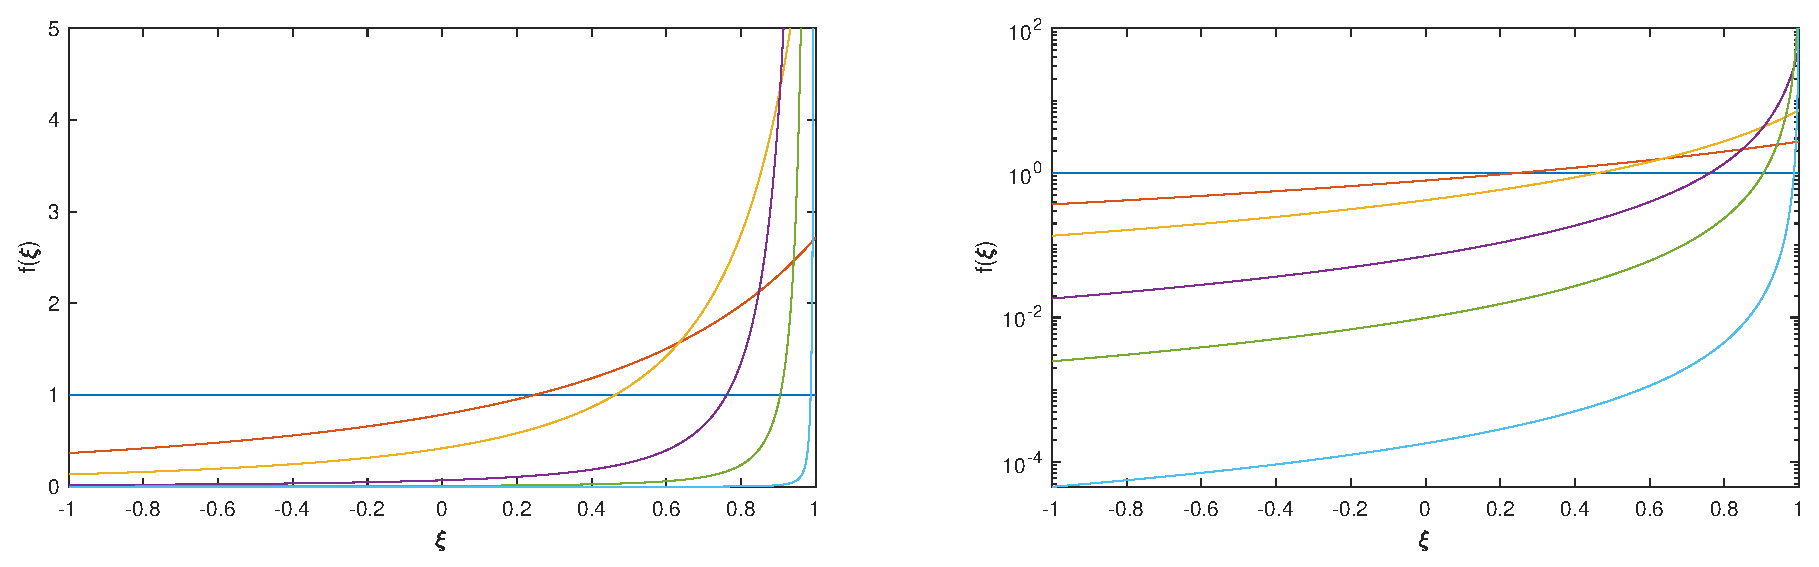
\includegraphics[scale=0.5]{FIGURES/fig_E_pitch}
%\label{fig_pitch_E_1}
\caption{Analytical solution of Eq.~(\ref{pitch_E_eq}) at 
$t=0$. 0.5, 1, 2 and 3 according to Eq.~(\ref{pitch_E_sol}) for initial condition $f_0=1$.}\label{Fig:Pitch_E_1}
\end{figure}

\vskip.1in
The error profiles and convergence results are reported in Table~\ref{Tab:Pitch_E-1}. One can observe that $L^2$-error converges at the order $\mathcal{O}(h^k)$ for central flux if $k$ is odd. In the case of employing $k=2$, we obtain super-convergence with rate around $\mathcal{O}(h^{k+1})$. By employing upwind flux, one can observe convergence rate $\mathcal{O}(h^{k+1/2})$, which is half order higher than that of using central flux for odd $k$. 

\begin{table}[H]
\caption{Test~\ref{SubSect:Pitch-1}: Error profiles and convergence test.}\label{Tab:Pitch_E-1}
\centering
\begin{tabular}{c|cc|cc}	\hline\hline
& \multicolumn{2}{c|}{CF} &\multicolumn{2}{c}{UF}\\ \hline
Lev & $\|f-f_h\|$ & Rate & $\|f-f_h\|$ & Rate \\ \hline		
&\multicolumn{4}{c}{$k=1$}\\ \hline
3	&1.5842E-01	&	        &3.4551E-02	& \\
4	&7.8928E-02	&1.01	&1.4192E-02	&1.28\\
5	&3.9003E-02	&1.02	&5.4647E-03	&1.38\\
6	&1.9405E-02	&1.01	&1.8316E-03	&1.58\\
7	&9.6866E-03	&1.00	&5.5644E-04	&1.72\\ \hline
			&\multicolumn{4}{c}{$k=2$}\\ \hline	
3	&1.5096E-02	&	&5.0869E-03	& \\
4	&1.9768E-03	&2.93	&1.0561E-03	&2.27\\
5	&1.7549E-04	&3.49	&2.3978E-04	&2.14\\
6	&1.2671E-05	&3.79	&4.4522E-05	&2.43\\
7	&8.4519E-07	&3.91	&7.1143E-06	&2.65\\ \hline
			&\multicolumn{4}{c}{$k=3$}\\ \hline	
3	&4.2329E-03	&	&8.0931E-04	& \\
4	&5.9217E-04	&2.84	&8.2762E-05	&3.29\\ 
5	&7.4760E-05	&2.99	&1.0673E-05	&2.96\\
6	&9.2476E-06	&3.02	&1.0853E-06	&3.30\\ 
7	&1.1471E-06	&3.01	&9.0918E-08	&3.58\\ \hline\hline
\end{tabular}
\end{table}

%------------------
% Figure
%------------------
\begin{figure}[H]
\begin{tabular}{cc}
  \includegraphics[width=.45\textwidth,height=.4\textwidth]{./NumFig/Test1-CF-L5D5}
  &\includegraphics[width=.45\textwidth,height=.4\textwidth]{./NumFig/Test1-UF-L5D5}\\
  (a) & (b)
  \end{tabular}
  \caption{Plot for numerical solutions for Lev = 5, $k = 4$ at $t = $ 0.5, 1, 2, 3: (a) central flux; (b) upwind flux.}\label{Fig:Pitch_E_1-Num2}
\end{figure}

Numerical experiment has been carried out on the mesh with Lev = 5, $k = 4$, and the numerical solutions are plotted in Figure~\ref{Fig:Pitch_E_1-Num2} for central flux and upwind flux. Since the solution approaches to a Dirac delta function centered at $\xi$, after several time steps, the numerical solution cannot capture the analytical solutions on the right end point. Thus, one begin to observe oscillations in the plot for both fluxes. Though the upwind flux cannot provide oscillation free scheme, the undershoots are around coordinate $1$. However, by using center flux, the numerical solution is oscillating in the whole domain.

%%------------------
%% Figure
%%------------------
%\begin{figure}[H]
%\begin{tabular}{cc}
%  \includegraphics[width=.45\textwidth,height=.4\textwidth]{./NumFig/Test1-CF-L5D5}
%  &\includegraphics[width=.45\textwidth,height=.4\textwidth]{./NumFig/Test1-UF-L5D5}\\
%  (a) & (b)
%  \end{tabular}
%  \caption{Plot for numerical solutions for Lev = 5, $k = 4$ at $t = $ 0.5, 1, 2, 3: (a) central flux; (b) upwind flux.}\label{Fig:Pitch_E_1-Num2}
%\end{figure}

\vskip.1in
\noindent{\bf Test~\ref{SubSect:Pitch-1}b} In this test, we set the initial condition as $f_0=\exp (-\xi^2/\sigma^2)$ with $\sigma=0.1$ and the solution is plotted in Figure~\ref{Fig:Pitch_E_2}. It is noted that, as shown in the figure, the solution asymptotically approaches a Dirac delta function centered at $\xi=1$.

Numerical experiment has been carried out on the mesh with Lev = 5, $k = 4$, and the numerical solutions are plotted in Figure~\ref{Fig:Pitch_E_2-Num2} for central flux and upwind flux.

%%%%%%%%%%%%%%%%%%%%%%%%%%%%%%%%%%%%%%%%%%%%
% FIGURE
%%%%%%%%%%%%%%%%%%%%%%%%%%%%%%%%%%%%%%%%%%%%
\begin{figure}[H]
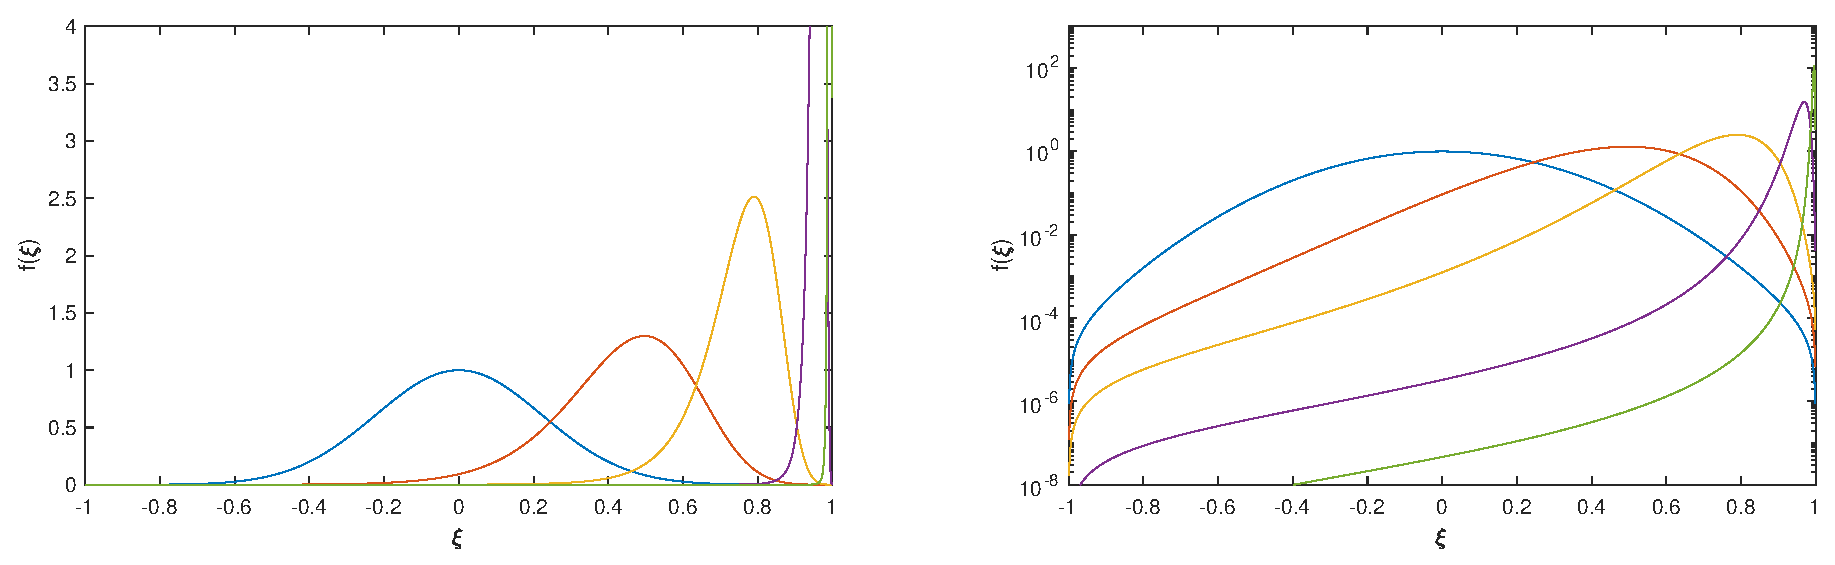
\includegraphics[scale=0.5]{FIGURES/fig_E_pitch_Gaussian}
%\label{fig_pitch_E_2}
\caption{Analytical solution of Eq.~(\ref{pitch_E_eq}) at 
$t=0$, 0.5, 1, 2 and 3 according to Eq.~(\ref{pitch_E_sol}) for initial condition $f_0=\exp(-\xi^2/\sigma^2)$.}\label{Fig:Pitch_E_2}
\end{figure}
%------------
% NumSol
%-------------
%%\begin{figure}[H]
%%\centering
%%\begin{tabular}{c}
%%  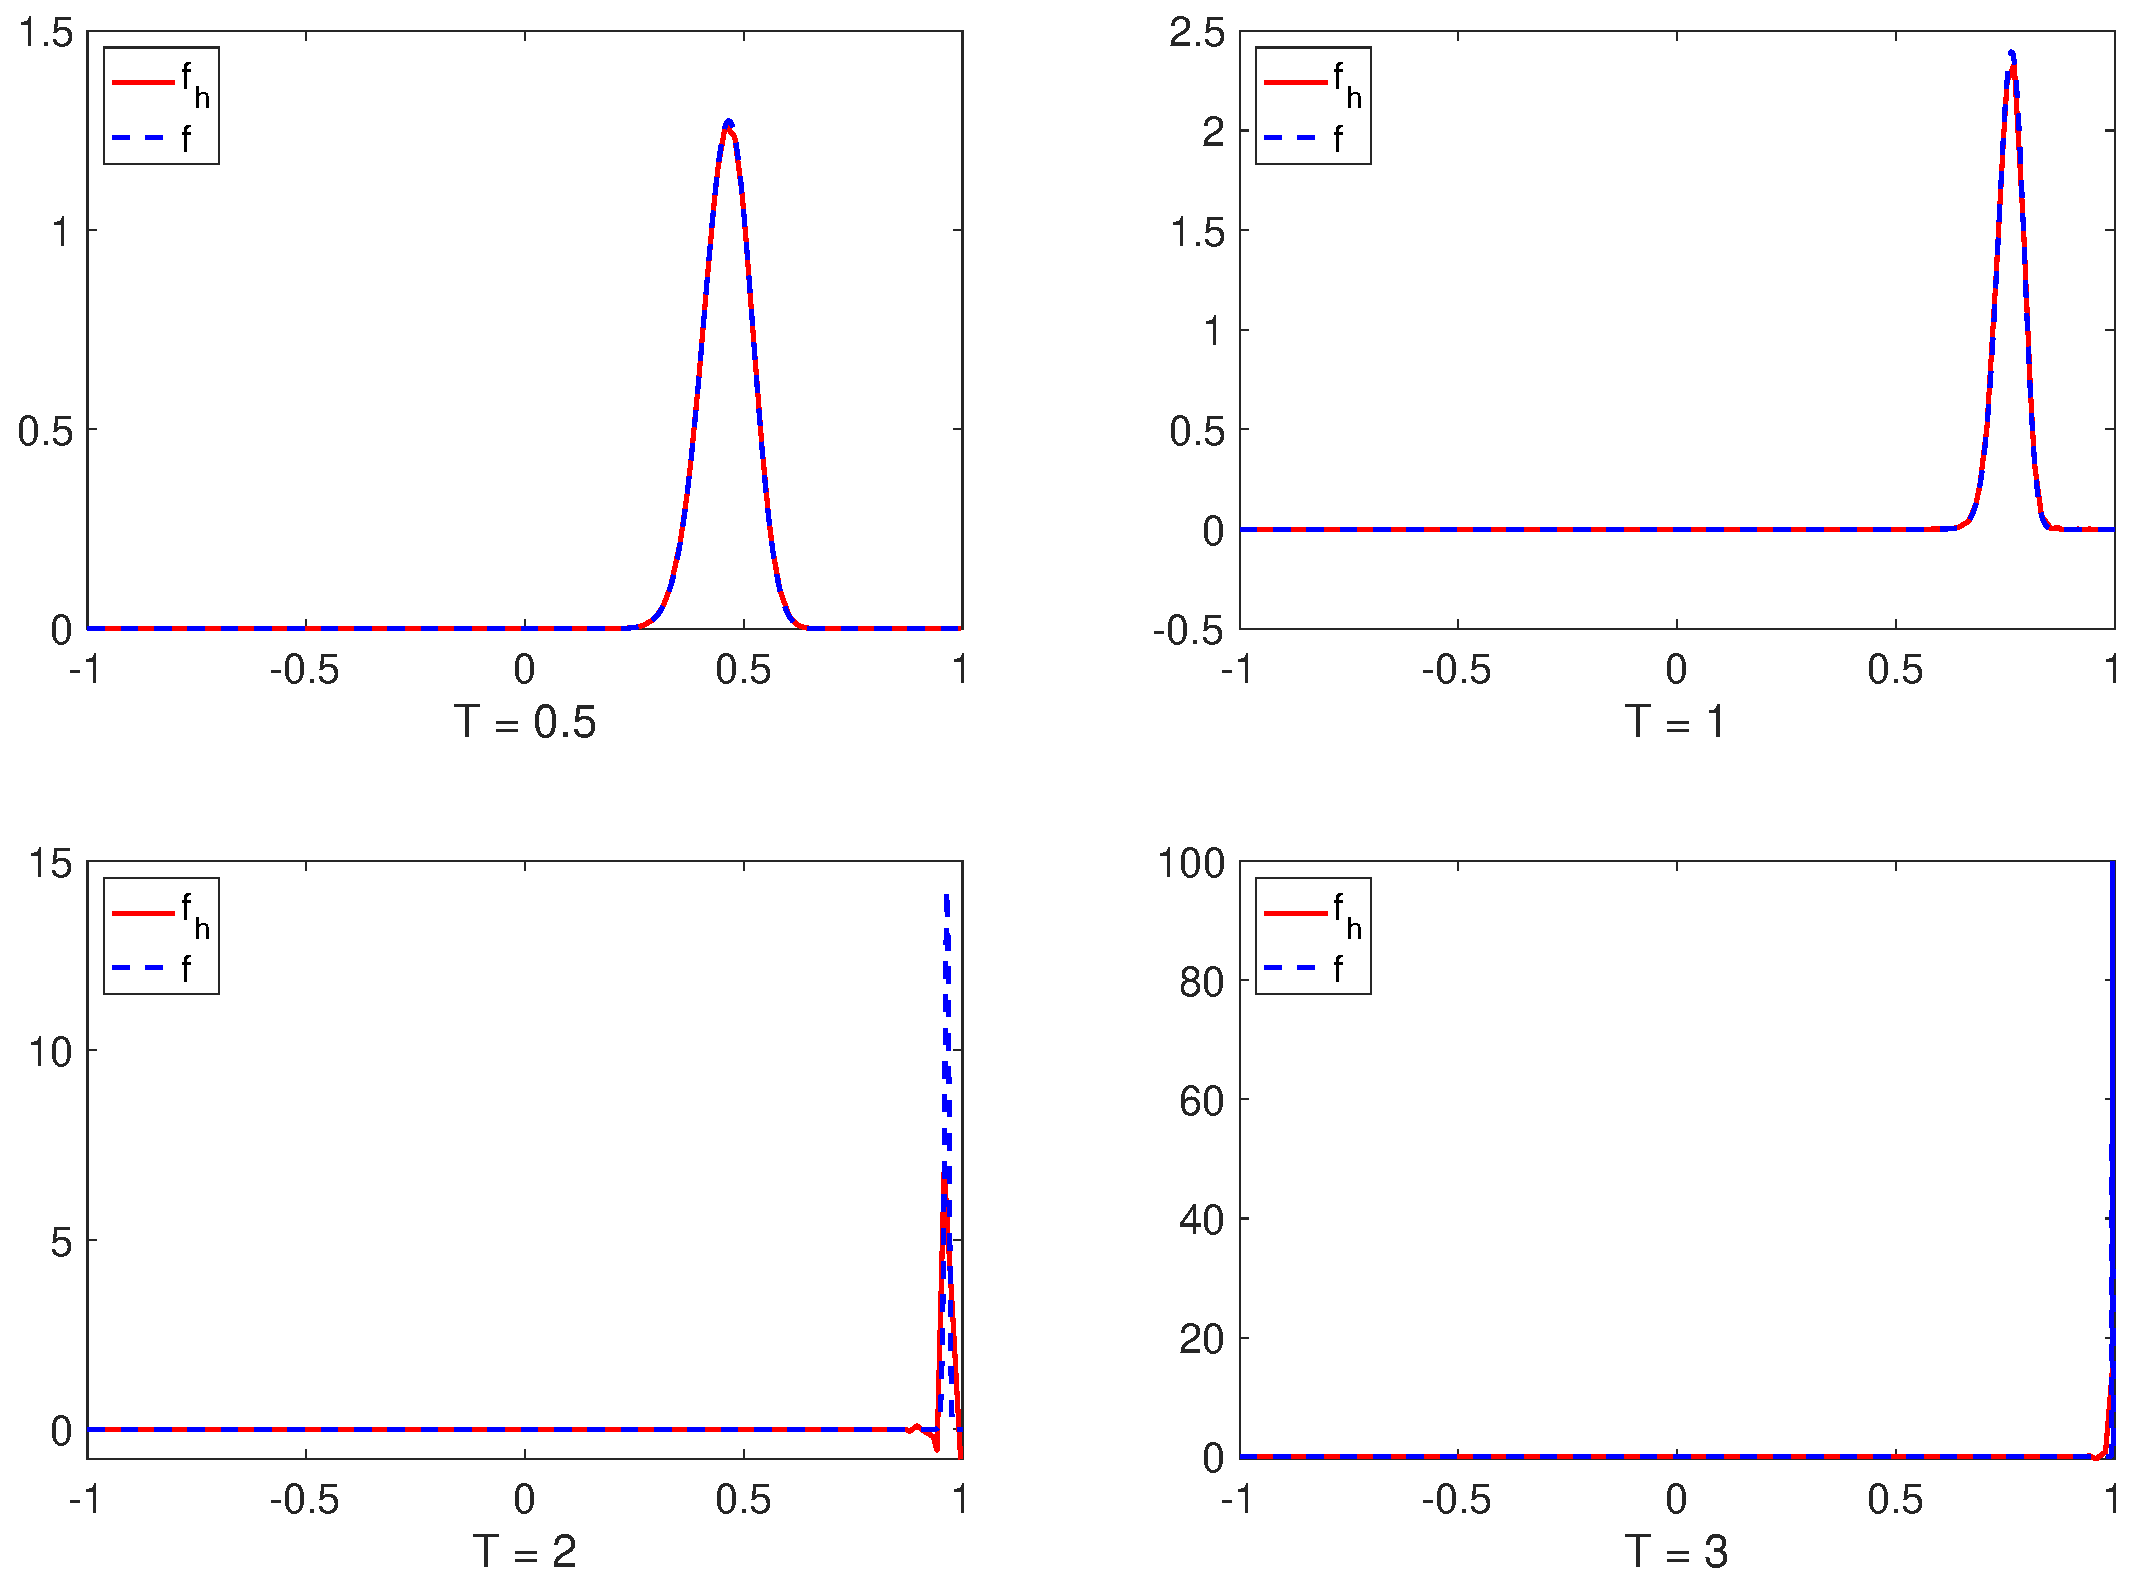
\includegraphics[width=.95\textwidth]{./NumFig/hyper-UF-Test2_v2}
%%  \end{tabular}
%%\caption{Plot for numerical solutions for Lev = 5, Deg = 5 of upwind flux at time = 0.5, 1, 2, 3.}
%%\label{Fig:Pitch_E_2-Num}
%%\end{figure}
%%%%%%%%%%%%%%%%%%%%%%%%%%%%%%%%%%%%%%%%%%%%%
\begin{figure}[H]
\begin{tabular}{cc}
  \includegraphics[width=.45\textwidth]{./NumFig/Test1-2-CF-L5D5}
  &\includegraphics[width=.45\textwidth]{./NumFig/Test1-2-UF-L5D5}\\
  (a) & (b)
  \end{tabular}
  \caption{Plot for numerical solutions for Lev = 5, $k = 4$ at $t = $ 0.5, 1, 2, 3: (a) central flux; (b) upwind flux.}\label{Fig:Pitch_E_2-Num2}
\end{figure}



\subsection{Collisions}\label{SubSect:Pitch-2}
%%%%%%%%%%%%%%%%%%%%%%%%%%%%%%%%%%%%%%%%%%%%%
The evolution of the pitch angle dependence of $f$ in the presence of only collisions is governed by the equation
\bq
\label{pitch_Coll_eq}
\frac{\partial f}{\partial t}= \frac{\partial}{\partial\xi} \left[ \left(1-\xi^2\right) \frac{\partial f}{\partial \xi} \right] \, ,
\eq
with initial and boundary conditions given in Eq.~(\ref{ic_bc}).
In this case the general solution is given by 
\bq
\label{pitch_Coll_sol}
 f(\xi, t)=\sum_{L=0}^\infty h_L P_L(\xi) e^{-L(L+1) t}\, ,
 \eq
where $P_L$ is the Legendre polynomial of degree $L$, and the coefficients $h_L$ are determined from the initial condition according to
\bq
\label{pitch_Coll_ic}
 f_0(\xi)=\sum_{L=0}^\infty h_L P_L(\xi)\, .
 \eq
 
 \noindent{\bf Test~\ref{SubSect:Pitch-2}} 
 In this test, we shall choose initial condition as (\ref{pitch_Coll_ic}) with $L=0,\dots,6$ and $h_0=3$,  $h_1=0.5$,  $h_2=1$,  $h_3=0.7$,  $h_4=3$,  $h_6=3$.
Figure~\ref{Fig:pitch_coll} (a) plots the solution for different time period.
% for the case $h_0=3$,  $h_1=0.5$,  $h_2=1$,  $h_3=0.7$,  $h_4=3$,  $h_6=3$,
%and all other  $h_L$ zero.  
%%%%%%%%%%%%%%%%%%%%%%%%%%%%%%%%%%%%%%%%%%%%
% FIGURE
%%%%%%%%%%%%%%%%%%%%%%%%%%%%%%%%%%%%%%%%%%%%
%\begin{figure}
%\begin{center}
%\includegraphics[scale=0.3]{FIGURES/fig_Coll_time-eps-converted-to}
%\end{center}
%\label{fig_pitch_coll}
%\caption{Analytical solution of Eq.~(\ref{pitch_Coll_eq}) at 
%$t=0.01$, 0.03, 0.05, 0.07 and 0.5 according to Eq.~(\ref{pitch_Coll_sol}) for initial condition in Eq.(\ref{pitch_Coll_ic}).}
%\end{figure}

%--------------
% Table
%-------------
\begin{table}[H]
\caption{Test~\ref{SubSect:Pitch-2}: Error profiles and convergence test of time = $0.03$.}\label{Tab:pitch_coll}
\centering
\begin{tabular}{c|cc|cc}	\hline\hline
Lev & $\|f-f_h\|_{\infty}$ & Rate & $\|f-f_h\|$ & Rate \\ \hline		
&\multicolumn{4}{c}{$k=1$}\\ \hline
2	&4.7098E-01	&	&2.0224E-01	&\\
3	&4.3233E-01	&0.12	&1.4733E-01	&0.46\\
4	&1.6836E-01	&1.36	&5.2630E-02	&1.49\\
5	&4.8070E-02	&1.81	&1.4376E-02	&1.87\\
6	&1.2284E-02	&1.97	&3.6140E-03	&1.99\\
7	&3.0468E-03	&2.01	&8.9771E-04	&2.01\\ \hline		
&\multicolumn{4}{c}{$k=2$}\\ \hline
2	&1.8990E-01	&	&1.0574E-01 &	\\
3	&5.4641E-02	&1.80	&2.4824E-02	&2.09\\
4	&9.7264E-03	&2.49	&3.3980E-03	&2.87\\
5	&1.2774E-03	&2.93	&4.1204E-04	&3.04\\
6	&1.5756E-04	&3.02	&5.0447E-05	&3.03\\
7	&1.9595E-05	&3.01	&6.2620E-06	&3.01\\ \hline		
&\multicolumn{4}{c}{$k=3$}\\ \hline
2	&3.8318E-02	&	&2.2665E-02	&\\
3	&3.8223E-03	&3.33	&1.7168E-03	&3.72\\
4	&2.6078E-04	&3.87	&1.0377E-04	&4.05\\
5	&1.6003E-05	&4.03	&6.3061E-06	&4.04\\
6	&9.8794E-07	&4.02	&3.9057E-07	&4.01\\
7	&6.1477E-08	&4.01	&2.4346E-08	&4.00\\ \hline\hline
\end{tabular}
\end{table}

The error profiles and convergence results to time period $0.03$ are reported in Table~\ref{Tab:pitch_coll}. The results show that the rate of convergence is at the order $\mathcal{O}(h^{k+1})$.
The analytical solutions and numerical solutions are plotted in Figure~\ref{Fig:pitch_coll}. As we running the simulation over longer time, the solution will approach to a flat line, and this is validated in our numerical experiment.




\begin{figure}[H]
\centering
\begin{tabular}{cc}
 \includegraphics[width=.45\textwidth]{FIGURES/fig_Coll_time-eps-converted-to}
  &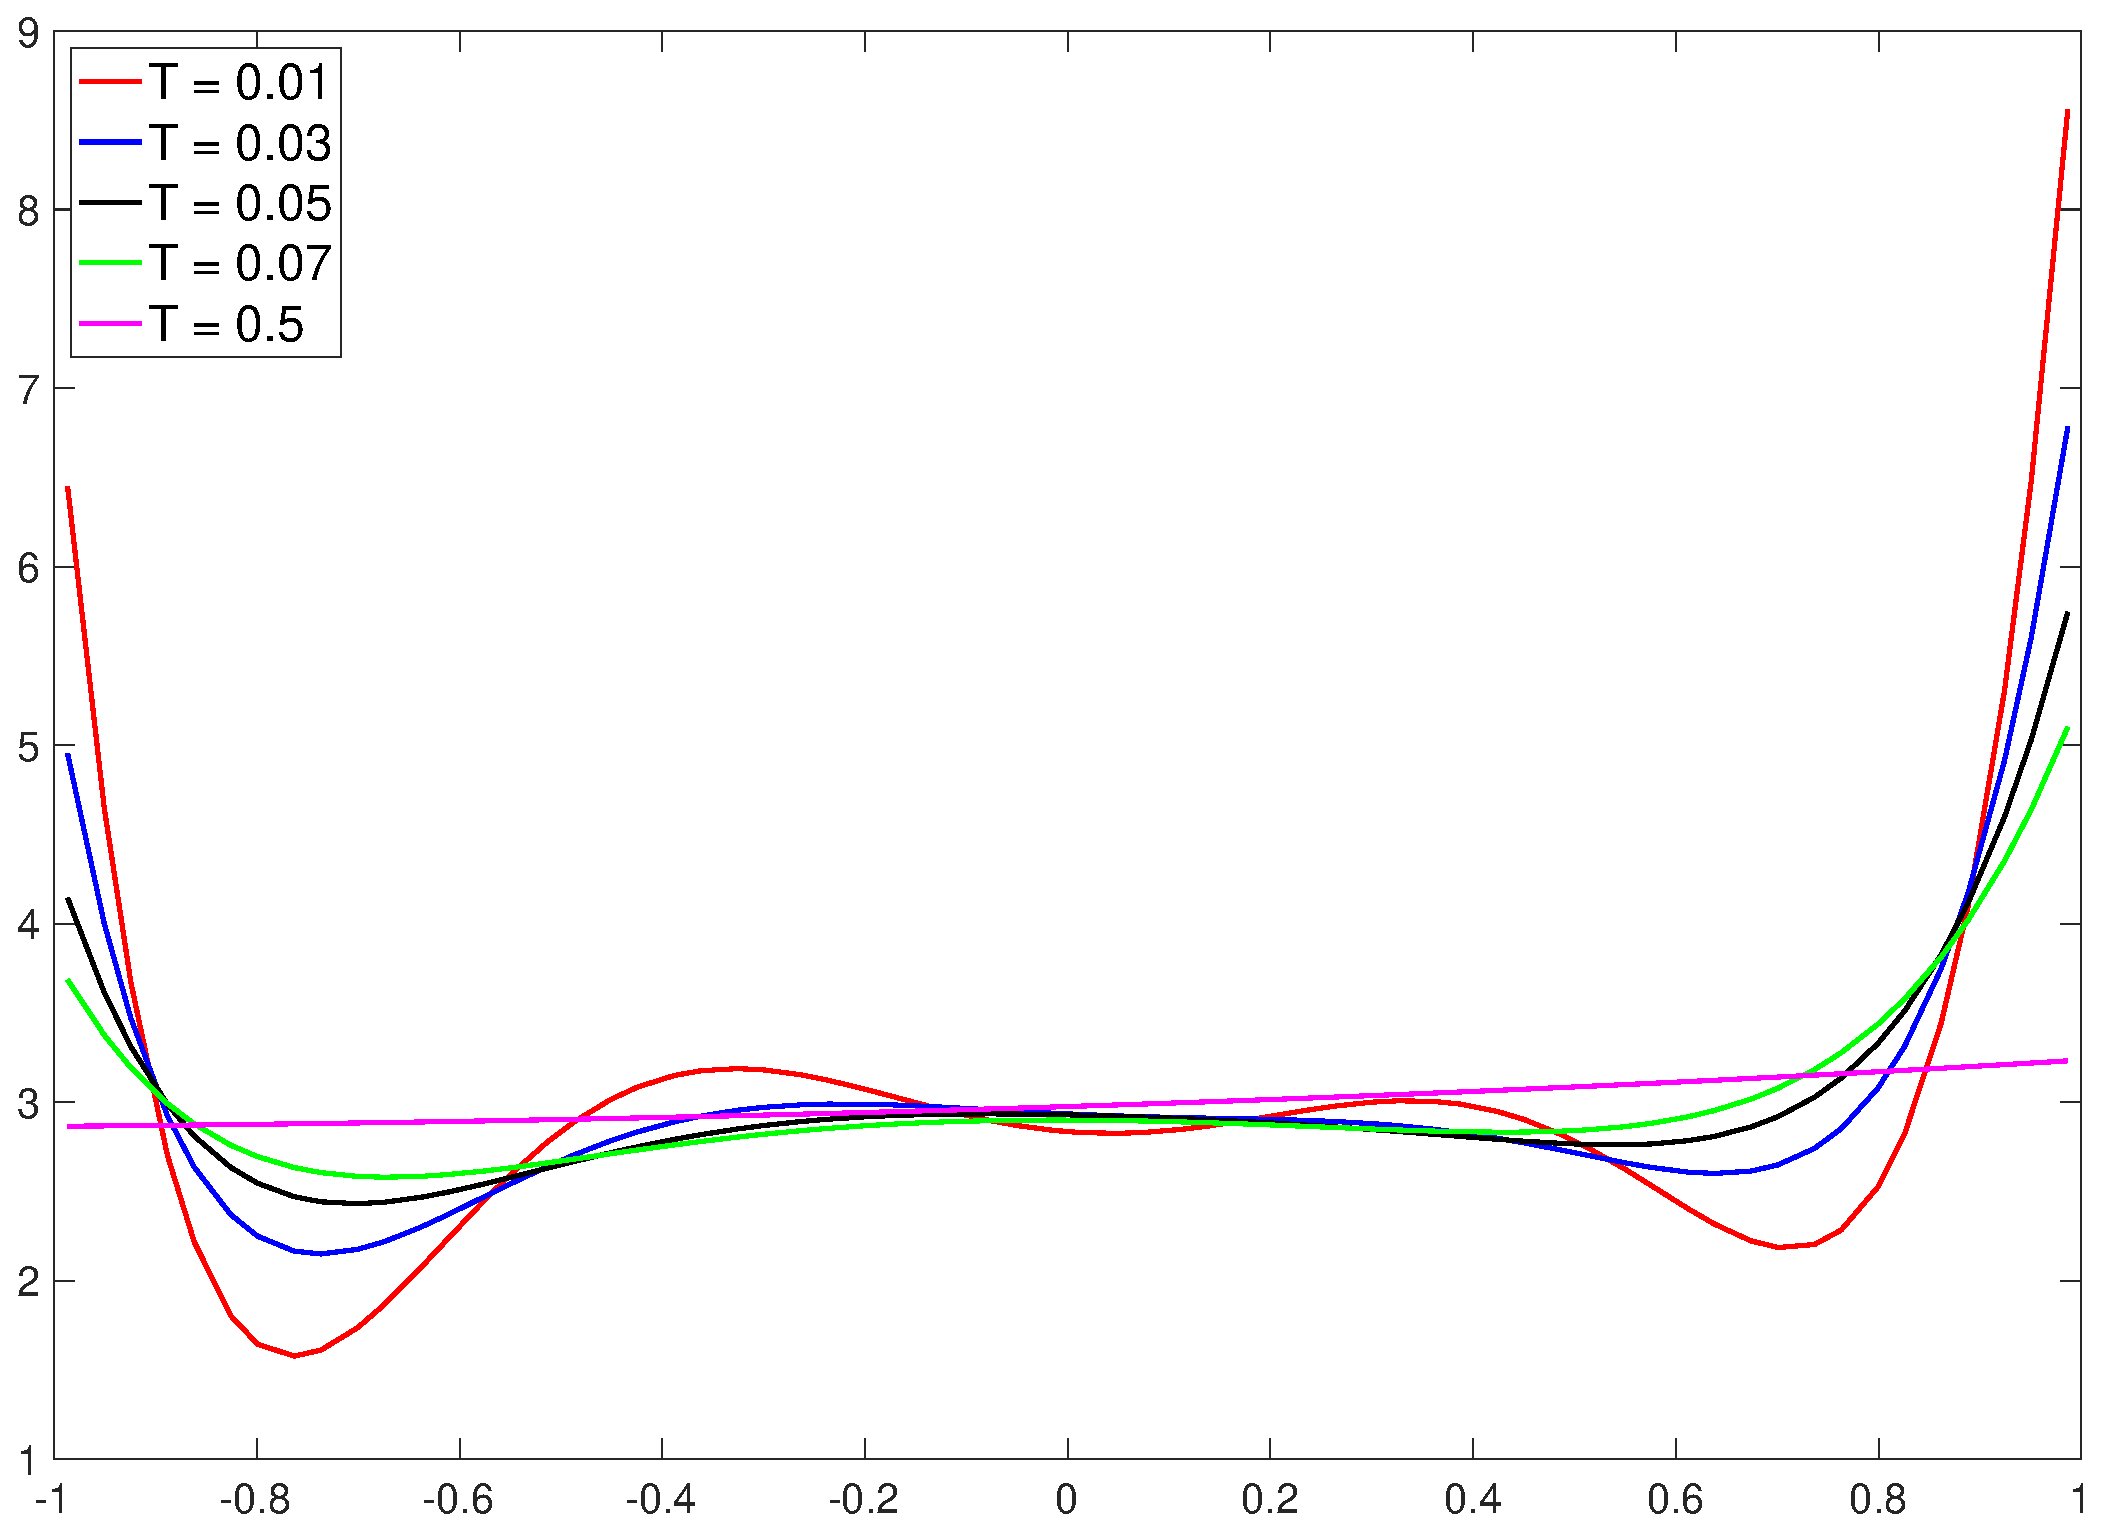
\includegraphics[width=.45\textwidth,height=.4\textwidth]{./NumFig/Diff-Deg5_Lev4}\\
  \footnotesize (a) & \footnotesize(b) 
\end{tabular}
\caption{(a) Analytical solution at 
$t=0.01$, 0.03, 0.05, 0.07 and 0.5 according to Eq.~(\ref{pitch_Coll_sol}); (b) Numerical solution with Lev = 4 and Deg = 5.}\label{Fig:pitch_coll}

\end{figure}

%%%%%%%%%%%%%%%%%%%%%%%%%%%%%%%%%%%%%%%%%%%%%
\subsection{Radiation damping}\label{SubSect:Pitch-3}
%%%%%%%%%%%%%%%%%%%%%%%%%%%%%%%%%%%%%%%%%%%%%
The evolution of the pitch angle dependence of $f$ in the presence of only radiation damping is governed by the equation
\bq
\label{pitch_Rad_eq}
\frac{\partial f}{\partial t}= -\frac{\partial}{\partial\xi} \left[\xi \left(1-\xi^2\right) f\right] \, ,
\eq
with initial and boundary conditions given in Eq.~(\ref{ic_bc}).
In this case the general solution is given by 
\bq
\label{pitch_Rad_sol}
f(\xi,t)=\frac{\phi \left ( 1- \phi^2\right)}{\xi \left(1-\xi^2\right)}\, f_0(\phi) \, ,
\eq
where
\bq
\phi=\frac{\xi e^{-t}}{\sqrt{1-\left(e^{-2t}-1\right) \xi^2}}\, .
\eq
%%Figure~\ref{fig:pitch_rad} shows examples of this solution for a centered Gaussian, shifted Gaussian and double Gaussian initial conditions. 
%%%%%%%%%%%%%%%%%%%%%%%%%%%%%%%%%%%%%%%%%%%%
% FIGURE
%%%%%%%%%%%%%%%%%%%%%%%%%%%%%%%%%%%%%%%%%%%%
%%\begin{figure}
%%\includegraphics[scale=0.4]{FIGURES/fig_rad_1}
%%\includegraphics[scale=0.4]{FIGURES/fig_rad_2}
%%\includegraphics[scale=0.4]{FIGURES/fig_rad_3}
%%\includegraphics[scale=0.4]{FIGURES/fig_rad_4}
%%\caption{Analytical solution of Eq.~(\ref{pitch_Rad_eq}) at 
%%different times according to Eq.~(\ref{pitch_Rad_sol}) for initial conditions: centered Gaussian, left-shifted Gaussian, right-shifted Gaussian and double Gaussian. Left (right) panels show solutions in linear (logarithmic) scale.}\label{fig:pitch_rad}
%%\end{figure}

\noindent{\bf Test~\ref{SubSect:Pitch-3}} In this test, we shall choose the function $f_0$ as Gaussian functions:
\begin{eqnarray*}
\text{Case 1.   }f_0 &=& \exp(-\frac{\xi^2}{\sigma^2}),\\
\text{Case 2.   }f_0 &=& \exp(-\frac{(\xi-0.36)^2}{\sigma^2}),\\
\text{Case 3.   }f_0 &=& \exp(-\frac{(\xi+0.36)^2}{\sigma^2}),\\
\text{Case 4.   }f_0 &=& \exp(-\frac{(\xi-0.36)^2}{\sigma^2})+\exp(-\frac{(\xi+0.36)^2}{\sigma^2}).\\
\end{eqnarray*}
%centered Gaussian and shifted Gaussian and double Gaussian as the initial conditions. The corresponding solutions are plotted in Figure~\ref{fig:pitch_rad}.

We perform the proposed numerical scheme in the simulation and the numerical results for Case 1 are reported in Table~\ref{Tab:pitch_rad}. It shows that error, measured in $\|\cdot\|_{\infty}$ and $\|\cdot\|$-norms, converges at the order $\mathcal{O}(h^{k+1})$. One can also observe super-convergence for $k=2$.

\begin{table}[H]
\caption{Test~\ref{SubSect:Pitch-3} (Case 1): Error profiles and convergence test at time$=3$.}\label{Tab:pitch_rad}
\centering
\begin{tabular}{c|cc|cc}	\hline\hline
Lev & $\|f-f_h\|_{\infty}$ & Rate & $\|f-f_h\|$ & Rate \\ \hline		
&\multicolumn{4}{c}{$k=1$}\\ \hline
3	&3.9497E-02	&	&2.3490E-02	& \\
4	&1.8914E-02	&1.06	&9.0040E-03	&1.38\\
5	&1.0083E-02	&0.91	&2.7059E-03	&1.73\\
6	&3.1273E-03	&1.69	&5.0826E-04	&2.41\\
7	&8.2423E-04	&1.92	&9.5484E-05	&2.41\\
8	&2.0879E-04	&1.98	&1.8460E-05	&2.37\\ \hline
	&\multicolumn{4}{c}{$k=2$}\\ \hline			
3	&2.5594E-02	&	&1.2153E-02	& \\
4	&1.0656E-02	&1.26	&3.3830E-03	&1.84\\
5	&1.1431E-03	&3.22	&3.1490E-04	&3.43\\
6	&8.2237E-05	&3.80	&2.6488E-05	&3.57\\
7	&6.6415E-06	&3.63	&1.7363E-06	&3.93\\
8	&4.8922E-07	&3.76	&1.0024E-07	&4.11\\ \hline
		&\multicolumn{4}{c}{$k=3$}\\ \hline		
3	&1.7571E-02	&	&7.5736E-03	& \\
4	&4.2588E-04	&5.37	&1.8950E-04	&5.32\\
5	&1.2814E-04	&1.73	&3.0874E-05	&2.62\\
6	&1.1815E-05	&3.44	&2.0460E-06	&3.92\\
7	&8.0768E-07	&3.87	&1.1012E-07	&4.22\\
8	&5.1717E-08	&3.97	&6.0220E-09	&4.19\\ \hline\hline
\end{tabular}
\end{table}


Then, we test our numerical scheme on the mesh with Lev$=8$ and $k=1$ and the numerical solutions are plotted in Figure~\ref{Fig:Pitch-3-1}-\ref{Fig:Pitch-3-4}. It is noted that our numerical scheme preserve mass through all the computation.

% NumFig
\begin{figure}[H]
\centering
\includegraphics[width=.32\textwidth]{./NumFig/Test4-3-1-L8D2}
\includegraphics[width=.32\textwidth]{./NumFig/Test4-3-1-L8D2-log}
\includegraphics[width=.32\textwidth]{./NumFig/Test4-3-k1-1-Con_v2}
\caption{Test~\ref{SubSect:Pitch-4}: Plots of numerical solutions at time $=0,0.5,1,2,3$ on mesh with Lev = 8, $k=1$: initial condition with centered Gaussian.}\label{Fig:Pitch-3-1}
\end{figure}

\begin{figure}[H]
\centering
\includegraphics[width=.32\textwidth]{./NumFig/Test4-3-3-L8D2}
\includegraphics[width=.32\textwidth]{./NumFig/Test4-3-3-L8D2-log}
\includegraphics[width=.32\textwidth]{./NumFig/Test4-3-k1-3-Con_v2}
\caption{Test~\ref{SubSect:Pitch-4}: Plots of numerical solutions at time $=0,0.5,1,2,3$ on mesh with Lev = 8, $k=1$: initial condition with left-shifted Gaussian.}\label{Fig:Pitch-3-2}
\end{figure}

\begin{figure}[H]
\centering
\includegraphics[width=.32\textwidth]{./NumFig/Test4-3-2-L8D2}
\includegraphics[width=.32\textwidth]{./NumFig/Test4-3-2-L8D2-log}
\includegraphics[width=.32\textwidth]{./NumFig/Test4-3-k1-2-Con_v2}
\caption{Test~\ref{SubSect:Pitch-4}: Plots of numerical solutions at time $=0,0.5,1,2,3$ on mesh with Lev = 8, $k=1$: initial condition with right-shifted Gaussian.}\label{Fig:Pitch-3-3}
\end{figure}

\begin{figure}[H]
\centering
\includegraphics[width=.32\textwidth]{./NumFig/Test4-3-4-L8D2}
\includegraphics[width=.32\textwidth]{./NumFig/Test4-3-4-L8D2-log}
\includegraphics[width=.32\textwidth]{./NumFig/Test4-3-k1-4-Con_v2}
\caption{Test~\ref{SubSect:Pitch-4}: Plots of numerical solutions at time $=0,0.5,1,2,3$ on mesh with Lev = 8, $k=1$: initial condition with double Gaussian.}\label{Fig:Pitch-3-4}
\end{figure}

%%%%%%%%%%%%%%%%%%%%%%%%%%%%%%%%%%%%%%%%%%%%%
\subsection{Electric field and collisions}\label{SubSect:Pitch-4}
%%%%%%%%%%%%%%%%%%%%%%%%%%%%%%%%%%%%%%%%%%%%%
The evolution of the pitch angle dependence of $f$ in the presence of electric field acceleration and collisions is governed by the equation
\bq
\label{pitch_E_coll_eq}
\frac{\partial f}{\partial t}= 
- E \frac{\partial}{\partial\xi} \left[ \left(1-\xi^2\right) f \right] + C \frac{\partial}{\partial\xi} \left[ \left(1-\xi^2\right) \frac{\partial f}{\partial \xi} \right]\, ,
\eq
with initial and boundary conditions given in Eq.~(\ref{ic_bc}).
%I could not find a time-dependent analytical solution in this case, but the steady-state, $\partial_t f=0$, solution is
%\bq
%\label{pitch_E_coll_sol}
%f(\xi)=\frac{A}{2 \sinh A} e^{A \xi}\, , \qquad A=E/C \, ,
%\eq
%where the pre-factor in the exponential is a normalization factor. Any normalized, $\int_{-1}^1 f_0 d \xi$, initial condition, asymptotically converges to the solution in Eq.~(\ref{pitch_E_coll_sol}). 
%

\noindent{\bf Test~\ref{SubSect:Pitch-4}} In this test, we shall use the following steady-state solution as the reference solution and check the proposed numerical scheme:
\bq
\label{pitch_E_coll_sol}
f(\xi)=\frac{A}{2 \sinh A} e^{A \xi}\, , \qquad A=E/C \, ,
\eq
where the pre-factor in the exponential is a normalization factor. Figure~\ref{fig_pitch_E_coll} illustrates the steady state solutions corresponding to different values in $A$.
%%%%%%%%%%%%%%%%%%%%%%%%%%%%%%%%%%%%%%%%%%%%
% FIGURE
%%%%%%%%%%%%%%%%%%%%%%%%%%%%%%%%%%%%%%%%%%%%
\begin{figure}[H]
\begin{center}
\includegraphics[scale=0.35]{FIGURES/fig_E_coll_std-eps-converted-to}
\end{center}
%\label{fig_pitch_rad}
\caption{Analytical steady state solution of Eq.~(\ref{pitch_E_coll_eq}) according to Eq.~(\ref{pitch_E_coll_sol}) for $A=1$, 2, 4, 6, 8, and 10.}\label{fig_pitch_E_coll}
\end{figure}


Let $C = 1$, the numerical solution for different $A$ are plotted in Figure~\ref{fig:pitch_E_coll}.

\begin{figure}[H]
\centering
\begin{tabular}{cc}
  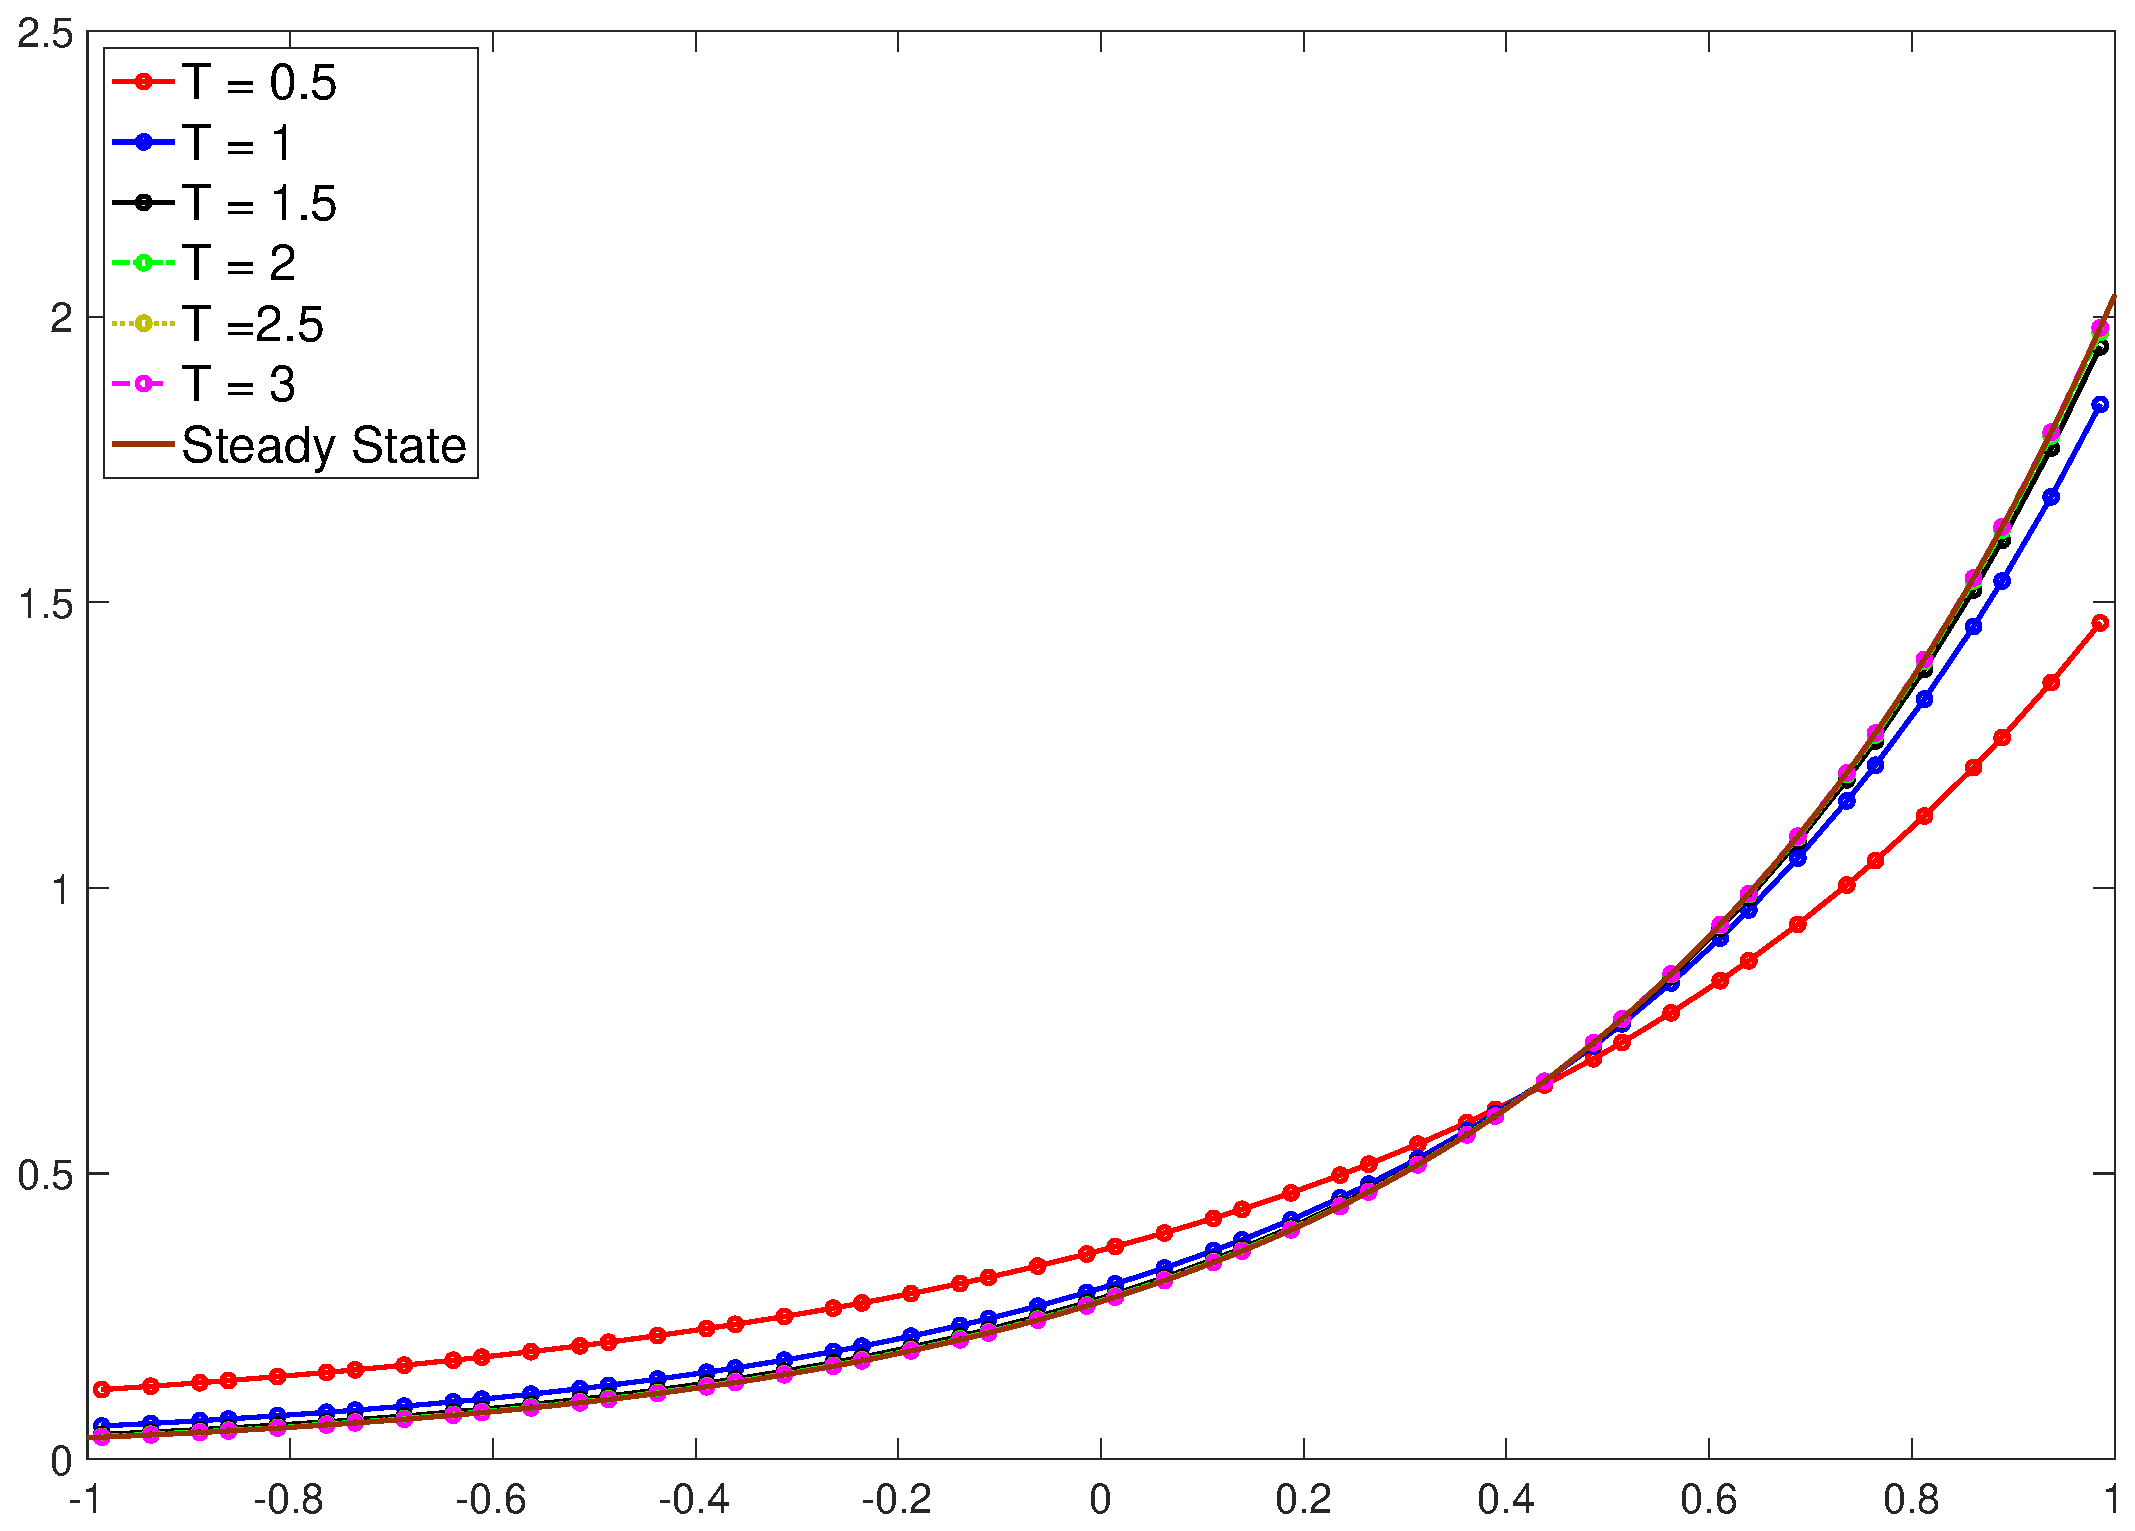
\includegraphics[width=.45\textwidth]{./NumFig/condiff-uf-E2_v2}
  &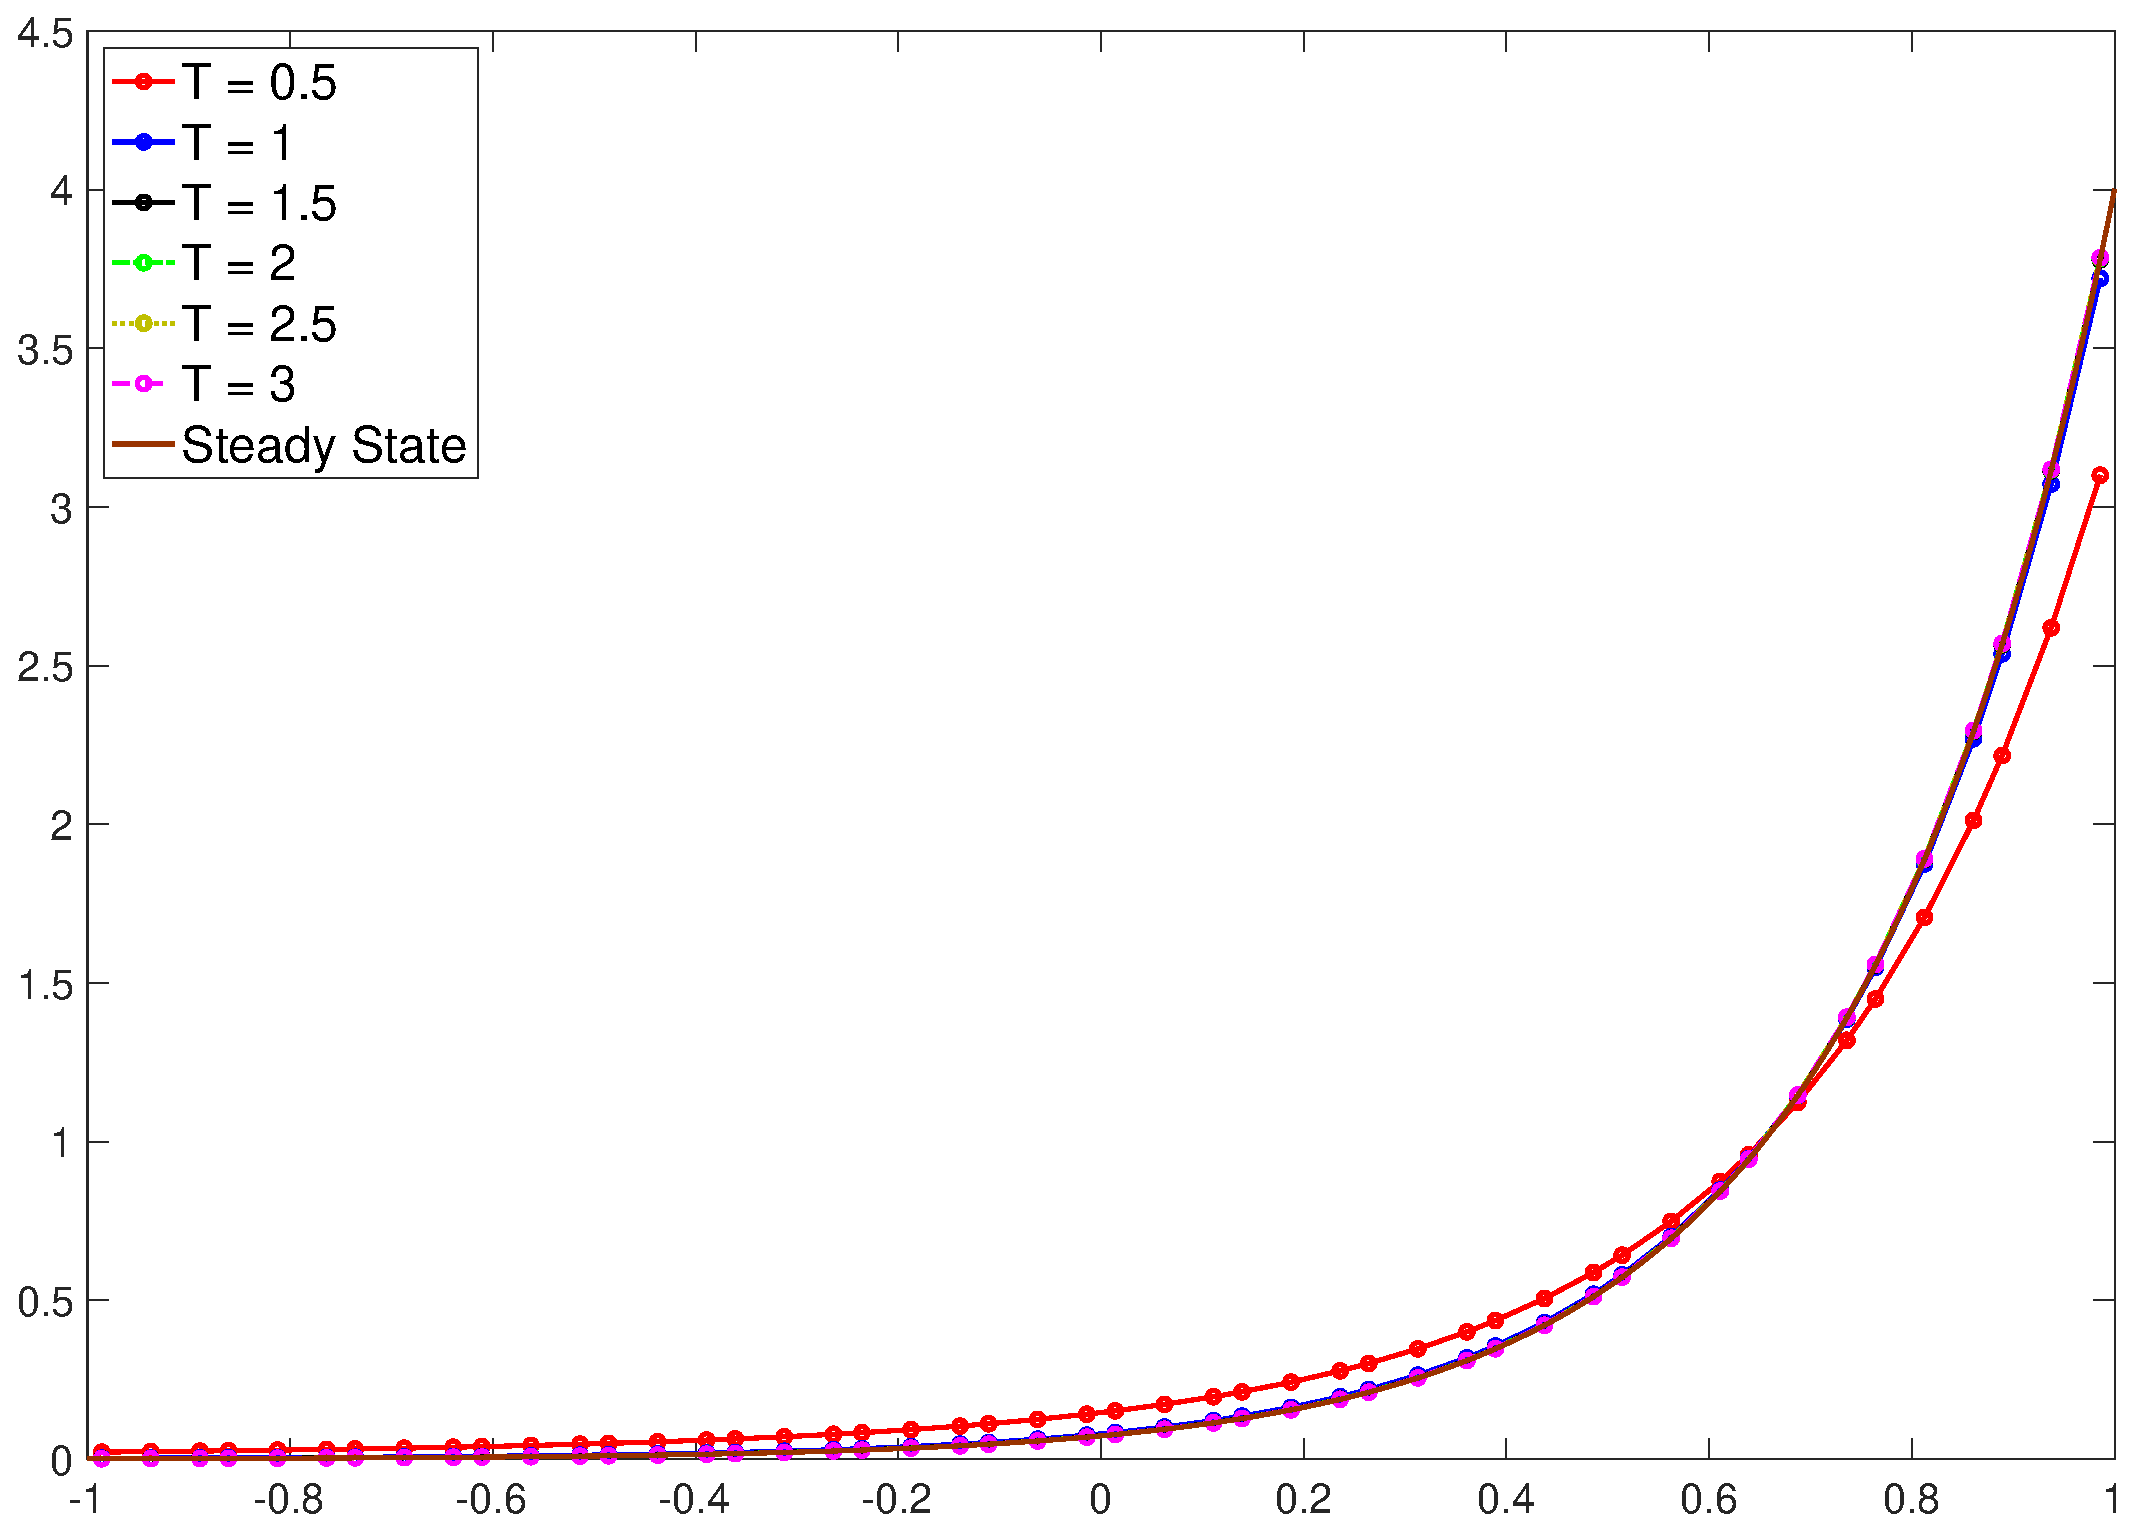
\includegraphics[width=.45\textwidth]{./NumFig/condiff-uf-E4_v2}\\
  (a) & (b)
  \end{tabular}
\caption{Plot for solutions for Lev = 4, $k = 4$ of upwind flux at time = 0.5, 1, 1.5, 2, 2.5, 3: (a) of $E=2$; (b) of $E = 4$.}\label{fig:pitch_E_coll}
\end{figure}



%%%%%%%%%%%%%%%%%%%%%%%%%%%%%%%%%%%%%%%%%%%%%
\subsection{Full pitch angle dynamics}\label{SubSect:Pitch-5}
%%%%%%%%%%%%%%%%%%%%%%%%%%%%%%%%%%%%%%%%%%%%%
The evolution of the pitch angle dependence of $f$ in the presence of electric field acceleration, collisions, and radiation damping is governed by the equation
\bq
\label{pitch_full_eq}
\frac{\partial f}{\partial t}= 
- E \frac{\partial}{\partial\xi} \left[ \left(1-\xi^2\right) f \right] + C \frac{\partial}{\partial\xi} \left[ \left(1-\xi^2\right) \frac{\partial f}{\partial \xi} \right] - R \frac{\partial}{\partial\xi} \left[\xi \left(1-\xi^2\right) f\right]  \, ,
\eq
where $E$, $C$, and $R$ are constants, and the initial and boundary conditions are given in Eq.~(\ref{ic_bc}). 
%In this case, the steady state solution is given by
%\bq
%\label{pitch_full_sol}
%f(\xi)= Q \exp \left[ {A\, \xi + (B/2) \, \xi^2}\right] \, , \qquad A=\frac{E}{C} \, , \qquad B=\frac{R}{C} \, ,
%\eq
%where $Q$ is a normalization constant. Figure~\ref{Fig:pitch_full} shows plots of this solution for different values of $E/C$ and $R/C$. 

\vskip.1in
\noindent{\bf Test~\ref{SubSect:Pitch-5}}
In this test, we shall use the following steady state solution as the reference solution for testing:
\bq
\label{pitch_full_sol}
f(\xi)= Q \exp \left[ {A\, \xi + (B/2) \, \xi^2}\right] \, , \qquad A=\frac{E}{C} \, , \qquad B=\frac{R}{C} \, ,
\eq
where $Q$ is a normalization constant. Figure~\ref{Fig:pitch_full} (a) and (b) show plots of this solution and numerical solutions for different values of $E/C$ and $R/C$.
%%%%%%%%%%%%%%%%%%%%%%%%%%%%%%%%%%%%%%%%%%%%
% FIGURE
%%%%%%%%%%%%%%%%%%%%%%%%%%%%%%%%%%%%%%%%%%%%
%\begin{figure}
%\begin{center}
%\includegraphics[scale=0.45]{FIGURES/fig_pitch_full}
%\end{center}
%\label{fig_pitch_full}
%\caption{Analytical steady state solution of Eq.~(\ref{pitch_full_eq}) according to Eq.~(\ref{pitch_full_sol}) different values of  $A=E/C=$, and $B=R/C$.}
%\end{figure}

\begin{figure}[H]
\centering
\begin{tabular}{cc}
 \includegraphics[width=.45\textwidth,height=.45\textwidth]{FIGURES/fig_pitch_full}
  &\includegraphics[width=.45\textwidth,height=.45\textwidth]{./NumFig/test_full}\\
  (a) & (b)
  \end{tabular}
\caption{(a) Analytical steady state solution of Eq.~(\ref{pitch_full_eq}) according to Eq.~(\ref{pitch_full_sol}) different values of  $A=E/C$, and $B=R/C$; (b) Corresponding numerical solutions.}\label{Fig:pitch_full}
\end{figure}

%%%%%%%%%%%%%%%%%%%%%%%%%%%%%%%%%%%%%%%%%%%%%
\section{Numerical Experiments of Momentum dynamics}\label{Sect:Mom}
%%%%%%%%%%%%%%%%%%%%%%%%%%%%%%%%%%%%%%%%%%%%%

The full, 1-D momentum dynamics is governed by the equation
\bq
\frac{\partial f}{\partial t}=\frac{1}{p^2} \frac{\partial}{\partial p} p^2 \left[ C_A \frac{\partial f}{\partial p} + C_F f\right]
 - \frac{E}{p^2} \, \frac{\partial}{\partial p}\, \left[ p^2 f\right] +
R \frac{1}{p^2} \frac{\partial}{\partial p}\left[ p^3 \gamma f \right] \, ,
\eq
with boundary conditions
\bq
\left. \frac{\partial f (p,t)}{\partial p}\right|_{p=0}=0 \, , \qquad f(p=p_{max},t)=0 \, ,
\eq
where $p_{max} \gg m v_{th}$. 
The steady-state solution of this equation is
\bq
f(p)=Q \exp \left[-\frac{1}{m T} \int \frac{p}{\sqrt{1+(p/mc)^2}} dp \right]
\exp \left[\int \left( \frac{E}{C_A} -\frac{R}{C_A} p  \sqrt{1+(p/mc)^2} \right) dp \right] \, ,
\eq
where $Q$ is a normalization constant, $m$ is the rest mass of the electron and $T$ the plasma temperature. 
In the non-relativistic limit, $p/mc\rightarrow 0$ and in the absence of electric field and radiation damping, $E=R=0$, the steady state reduces to the expected Maxwellian distribution 
\bq
\label{eq_maxwell}
f(p)=Q \exp \left[-\frac{p^2}{2m T} \right]= Q \exp \left[-\left(\frac{v}{v_{th}}\right)^2 \right] \, ,
\eq
where $v_{th}=\sqrt{2 T/m}$ is the plasma thermal temperature. 
\subsection{Collisions}\label{SubSect:mom-collisions}
As an starting point we should check that the numerical solution converges to the Maxwellian in the non-relativistic limit with $E=R=0$. That is, reduce the problem to the solution of
\bq
\frac{\partial f}{\partial t}=\frac{1}{p^2} \frac{\partial}{\partial p} p^2 \left[ C_A \frac{\partial f}{\partial p} + C_F f\right] \, .
\eq
%For the numerical test it would be convenient to use the non-dimensional variable $x=v/v_{th}$, rescale the time $t$, and write the Fokker-Planck equation as
%\bq
%\frac{\partial f}{\partial t}=\frac{1}{x^2} \frac{\partial}{\partial x} x^2 \left[ \frac{\psi(x)}{x}\frac{\partial f}{\partial p} + 2 \psi(x) f\right] \, ,
%\eq
%where we have used Eqs.~(\ref{coll_eq_1}) and (\ref{coll_eq_3}) and $\psi(x)$ is defined in Eq.~(\ref{coll_fcns}). The boundary conditions are
%\bq
%\left. \frac{\partial f (x,t)}{\partial x}\right|_{x=0}=0 \, , \qquad f(x=x_{max},t)=0 \, ,
%\eq
%where $x_{max} \gg 1$. In these variables, according to Eq.~(\ref{eq_maxwell}) the steady state is simply $f(x)=Q e^{-x^2}$. 

\vspace{10pt}
\noindent{\bf Test~\ref{SubSect:mom-collisions}a}. In this test, we will use the non-dimensional variable $x=v/v_{th}$, rescale the time $t$, and write the Fokker-Planck equation as
\bq
\frac{\partial f}{\partial t}=\frac{1}{x^2} \frac{\partial}{\partial x} x^2 \left[ \frac{\psi(x)}{x}\frac{\partial f}{\partial x} + 2 \psi(x) f\right] \, ,
\eq
where $\psi(x)$ is defined as
\begin{eqnarray}
\phi(x)=\mathrm{erf}(x)=\frac{2}{\sqrt{\pi}}\int_0^x e^{-s^2}ds,\ \psi(x)=\frac{1}{2x^2}\bigg(\phi(x)-x\frac{d\phi}{dx}\bigg).
\end{eqnarray}
The boundary conditions are
\bq
\left. \frac{\partial f (x,t)}{\partial x}\right|_{x=0}=0 \, , \qquad f(x=x_{\max},t)=0 \, ,
\eq
where $x_{\max} \gg 1$. In these variables, according to Eq~(\ref{eq_maxwell}) the steady state is simply $\frac{4}{\sqrt{\pi}}e^{-x^2}$.%$f(x)=Q e^{-x^2}$. 
The numerical experiment is carried out by assuming $x_{\max}=10.$

\begin{itemize}
\item The first test is to choose initial condition as $\frac{4}{\sqrt{\pi}a^3}e^{-x^2/a^2}$ and set $a=2$.
In this test, we run the numerical simulation until the difference of $f^{n-1}$ and $f^n$ is less than $10^{-10}$ and this requires the end time as $340$. The comparison of numerical solution at $time = 340$ with steady state is reported in Table~\ref{Tab:Mom-1}. It can be observed that the rate for convergence is $\mathcal{O}(h^{k+1})$. In the cubic element's simulation, $10^{-10}$ is not enough for chosen as the approximation of steady state and when lev is bigger than 8, the optimal convergence rate can not be preserved.
\begin{figure}[H]
\centering
\includegraphics[width=.48\textwidth]{./NumFig/Ini-Mom-1}
\includegraphics[width=.48\textwidth]{./NumFig/Ini-Mom-1-Conv.png}
\caption{Test~\ref{Sect:Mom}: Plot of numerical solution.}\label{Fig:Mom-1}
\end{figure}

\begin{table}[H]
\caption{Test~\ref{Sect:Mom}: Error profiles and convergence test.}\label{Tab:Mom-1}
\centering
\begin{tabular}{c|cc|cc}	\hline\hline
Lev & $\|f-f_h\|_{\infty}$ & Rate & $\|f-f_h\|$ & Rate \\ \hline		
&\multicolumn{4}{c}{$k=1$}\\ \hline
4	&5.2864E-02	&		&5.2892E-02	&\\
5	&2.5388E-02	&1.06	&1.4358E-02	&1.88\\
6	&6.5526E-03	&1.95	&3.6769E-03	&1.97\\
7	&1.5249E-03	&2.10	&9.1786E-04	&2.00\\
8	&3.5857E-04	&2.09	&2.2854E-04	&2.01\\
9	&8.6355E-05	&2.05	&5.6976E-05	&2.00\\
10	&2.1152E-05	&2.03	&1.4222E-05	&2.00\\ \hline
&\multicolumn{4}{c}{$k=2$}\\ \hline		
4	&9.1049E-03	&		&7.4916E-03	&\\
5	&1.1269E-03	&3.01	&8.7676E-04	&3.10\\
6	&1.4136E-04	&2.99	&1.0205E-04	&3.10\\
7	&1.7600E-05	&3.01	&1.2460E-05	&3.03\\
8	&2.1939E-06	&3.00	&1.5457E-06	&3.01\\
9	&2.7141E-07	&3.01	&1.9264E-07	&3.00\\
10	&3.1662E-08	&3.10	&2.4195E-08	&2.99\\ \hline
&\multicolumn{4}{c}{$k=3$}\\ \hline				
4	&6.7085E-04	&		&5.3862E-04	&\\
5	&4.7544E-05	&3.82	&3.6259E-05	&3.89\\
6	&3.6905E-06	&3.69	&2.4362E-06	&3.90\\
7	&2.4618E-07	&3.91	&1.5398E-07	&3.98\\
8	&1.8430E-08	&3.74	&9.9121E-09	&3.96\\
9	&4.0258E-09	&2.19	&2.4803E-09	&2.00\\
10	&4.2010E-09	&-       	&3.2612E-09	&- \\ \hline
\hline
\end{tabular}
\end{table}

\item The second test is to choose initial condition as 
$$
f = \begin{cases}
\frac{3}{5^3},\ x\in[0,5],\\
0,\text{ else}.
\end{cases}
$$
Similarly, we will conduct the numerical simulation until the difference for $f^{n-1}$ and $f^n$ is less than $10^{-10}$ and thus choose the end time as $230$. The comparison of numerical solution at $time = 230$ with steady state is reported in Table~\ref{Tab:Mom-2}. It can be observed that the rate for convergence is $\mathcal{O}(h^{k+1})$. In the cubic element's simulation, $10^{-10}$ is not enough for chosen as the approximation of steady state and when lev is bigger than 8, the optimal convergence rate can not be preserved.
\begin{figure}[H]
\centering
\begin{tabular}{ccc}
\includegraphics[width=.3\textwidth]{./NumFig/Ini-Mom-2-zoom}
&\includegraphics[width=.3\textwidth]{./NumFig/Ini-Mom-2}
&\includegraphics[width=.3\textwidth]{./NumFig/Ini-Mom-2-Conv.png}\\
(a) & (b) & (c)
\end{tabular}
\caption{Test~\ref{Sect:Mom}: Plot of numerical solution.}\label{Fig:Mom}
\end{figure}
\end{itemize}

\begin{table}[H]
\caption{Test~\ref{Sect:Mom}: Error profiles and convergence test.}\label{Tab:Mom-2}
\centering
\begin{tabular}{c|cc|cc}	\hline\hline
Lev & $\|f-f_h\|_{\infty}$ & Rate & $\|f-f_h\|$ & Rate \\ \hline		
&\multicolumn{4}{c}{$k=1$}\\ \hline
4	&5.2865E-02	&		&5.2892E-02	&\\
5	&2.5388E-02	&1.06	&1.4358E-02	&1.88\\
6	&6.5526E-03	&1.95	&3.6769E-03	&1.97\\
7	&1.5249E-03	&2.10	&9.1786E-04	&2.00\\
8	&3.5858E-04	&2.09	&2.2854E-04	&2.01\\
9	&8.6356E-05	&2.05	&5.6976E-05	&2.00\\
10	&2.1154E-05	&2.03	&1.4222E-05	&2.00 \\ \hline		
&\multicolumn{4}{c}{$k=2$}\\ \hline
4	&9.1049E-03	&		&7.4916E-03	&\\
5	&1.1269E-03	&3.01	&8.7676E-04	&3.10\\
6	&1.4137E-04	&2.99	&1.0205E-04	&3.10\\
7	&1.7602E-05	&3.01	&1.2460E-05	&3.03\\
8	&2.1953E-06	&3.00	&1.5456E-06	&3.01\\
9	&2.7289E-07	&3.01	&1.9263E-07	&3.00\\
10	&3.3138E-08	&3.04	&2.4072E-08	&3.00 \\ \hline		
&\multicolumn{4}{c}{$k=3$}\\ \hline
4	&6.7084E-04	&		&5.3862E-04	&\\
5	&4.7546E-05	&3.82	&3.6259E-05	&3.89\\
6	&3.6887E-06	&3.69	&2.4361E-06	&3.90\\
7	&2.4439E-07	&3.92	&1.5396E-07	&3.98\\
8	&1.6609E-08	&3.88	&9.6664E-09	&3.99\\
9	&2.1963E-09	&2.92	&1.1318E-09	&3.09\\
10	&1.8878E-09	&-	&1.4318E-09	&- \\ \hline
\hline
\end{tabular}
\end{table}

%\vskip.1in
%Numerical solution is plotted in Figure~\ref{Fig:Mom}.

%\begin{figure}
%\centering
%\includegraphics[width=.48\textwidth]{./NumFig/Test5-Q}
%\caption{Test~\ref{Sect:Mom}: Plot of numerical solution.}\label{Fig:Mom}
%\end{figure}
%%%%%%%%%%%%%%%%%%%%%%%%%%%%%%%%%%%%%%%%%%%%%
\section{Numerical Experiments of Full 2D dynamics}\label{Sect:FullModel}
%%%%%%%%%%%%%%%%%%%%%%%%%%%%%%%%%%%%%%%%%%%%%

As an starting point we will assume a time-independent plasma density and temperature, 
\bq
{\tilde T}=T \, , \qquad {\tilde n}=n \, ,
\eq
which implies 
\bq
 \bar{\nu}_{ee}=1 \, , \qquad \bar{v}_T=1 \, .
 \eq
% In this case, the model parameters are $\delta$, $Z$, $\hat{\tau}$, and $\hat{E}$.
% To test the code we can try
%\bq
%\delta=0.042 \, , \qquad Z=1 \, , \qquad {\hat E}=0.0025 \, , \qquad \hat{\tau}=10^5 \, ,
%\eq
%with integration time $t_{max}=10^3$ and  momentum domain $\hat{p} \in (0,10)$. 
%For the initial condition we will take a Maxwellian distribution
%\bq
%f= \frac{2}{\sqrt \pi} e^{-{\hat p}^2} \, , \qquad \int_{-\xi}^\xi\,  d \xi  \int_{0}^\infty \, f \, {\hat p}^2 \, d {\hat p} =1  
%\eq
\subsection{Collison Term $\Gamma^C$}
\noindent{\bf Test~\ref{Sect:FullModel}.}
 In this test, we set the model parameters as% $\delta$, $Z$, $\hat{\tau}$, and $\hat{E}$.
 %To test the code we can try
\bq
\delta=0.042 \, , \qquad Z=1 \, , \qquad {\hat E}=0.0025 \, , \qquad \hat{\tau}=10^5 \, ,
\eq
with integration time $t_{max}=10^3$, and let domain $\xi\times\hat{p}\in [-1,1]\times[0,10]$.
For the initial condition we will take a Maxwellian distribution
\bq
f= \frac{2}{\sqrt \pi} e^{-{\hat p}^2} \, , \qquad \int_{-1}^1\,  d \xi  \int_{0}^\infty \, f \, {\hat p}^2 \, d {\hat p} =1.  
\eq
The boundary conditions are: Neumann boundary for $\xi$ and 
\begin{eqnarray*}
\left. \frac{\partial f}{\partial \hat{p}}\right|_{\hat{p}=0}=0 \, , \qquad f(\hat{p}=10,t)=0
\end{eqnarray*}


%
%\begin{figure}[H]
%\centering
%\includegraphics[width=.48\textwidth]{./NumFig/Test_2D_Ini}
%\caption{Test~\ref{Sect:FullModel}: Plot of initial condition.}
%\end{figure}

\begin{figure}[H]
\centering
\includegraphics[width=.32\textwidth]{./NumFig/FullModel-Ca}
\includegraphics[width=.32\textwidth]{./NumFig/FullModel-Cb}
\includegraphics[width=.32\textwidth]{./NumFig/FullModel-Cf}
\caption{Test~\ref{Sect:FullModel}: Plot of coefficients $C_A$ (left), $C_B$ (middle), and $C_F$ (right).}
\end{figure}

In the first test, we shall consider the term $\Gamma^c$ and the equation is described as follows:
\begin{eqnarray*}
\frac{\partial f}{\partial t} = \frac{1}{{\hat p}^2}\frac{\partial}{\partial {\hat p}}\bigg({\hat p}^2C_A\frac{\partial f}{\partial {\hat p}}\bigg) + \frac{1}{{\hat p}^2}\frac{\partial}{\partial {\hat p}}\bigg({\hat p}^2C_F f\bigg)+\frac{1}{{\hat p}^4}\frac{\partial}{\partial\xi}\bigg(C_B(1-\xi^2)\frac{\partial f}{\partial\xi}\bigg).
\end{eqnarray*}
The initial condition is set as $f= \frac{2}{\sqrt \pi} e^{-{\hat p}^2}$.

\begin{itemize}
\item Method 1
\begin{eqnarray}
\hat{p}^2\frac{\partial f}{\partial t} = \frac{\partial}{\partial {\hat p}}\bigg({\hat p}^2C_A\frac{\partial f}{\partial {\hat p}}\bigg) + \frac{\partial}{\partial {\hat p}}\bigg({\hat p}^2C_F f\bigg)+\frac{1}{{\hat p}^2}\frac{\partial}{\partial\xi}\bigg(C_B(1-\xi^2)\frac{\partial f}{\partial\xi}\bigg).
\end{eqnarray}
\item Method 2: Truncate the domain and let $\hat{p}\in(I_t,10)$.
\end{itemize}
When we exam Method 1, 


\begin{figure}[H]
\centering
\includegraphics[width=.32\textwidth]{./NumFig/Test_2D_Eig_L2D2}
\includegraphics[width=.32\textwidth]{./NumFig/Test_2D_Eig_L3D2}
\includegraphics[width=.32\textwidth]{./NumFig/Test_2D_Eig_L4D2}
\caption{Test~\ref{Sect:FullModel}: Plot of eigenvalues for $k = 1$ and Lev $= 2$ (left), Lev $= 3$ (middle), Lev $= 4$ (right).}
\end{figure}

\begin{figure}[H]
\centering
\includegraphics[width=.32\textwidth]{./NumFig/Test_2D_Eig_L4_1e-2}
\includegraphics[width=.32\textwidth]{./NumFig/Test_2D_Eig_L4_1e-1}
\includegraphics[width=.32\textwidth]{./NumFig/Test_2D_Eig_L4_5e-1}
\caption{Test~\ref{Sect:FullModel}: Plot of eigenvalues of $k = 1$ and Lev $= 4$ for $(0.01,10)$ (left), $(0.1,10)$ (middle), and $(0.5,10)$ (right).}
\end{figure}

\noindent{\bf Test~\ref{Sect:FullModel}-1}
The initial condition is chosen as
\begin{eqnarray}
f_0(\xi,\hat{p},t=0) = \begin{cases}
\dfrac{3}{2\cdot5^3}, \text{ if }0\le \hat{p}\le5,\\
0,\text{ else}.
\end{cases}\label{NumTest6-1}
\end{eqnarray}
Figure~\ref{Fig:NumTest6-1-1} plots the numerical solution at the mesh with Lev = $5$, $k=1$. At $t=0$, the solution is step function in $\hat{p}$. After 

% Test1
\begin{figure}[H]
\centering
\includegraphics[width=.32\textwidth]{./NumFig/FullModel2D-1-Ini}
\includegraphics[width=.32\textwidth]{./NumFig/FullModel2D-1-100}
\includegraphics[width=.32\textwidth]{./NumFig/FullModel2D-1-Conv}
\caption{Test~\ref{Sect:FullModel}: Plot of initial condition (\ref{NumTest6-1}) (left), solution at time $= 100$ (middle), and conservation property (right).}\label{Fig:NumTest6-1-1}
\end{figure}

% Test 2
\noindent{\bf Test~\ref{Sect:FullModel}-2}
The initial condition is chosen as
\begin{eqnarray}
f_0(\xi,\hat{p}) = \frac{2}{\sqrt{\pi}a^3}\exp(-\hat{p}^2/a^2), \text{ with } a = 2.\label{NumTest6-2}
\end{eqnarray}

\begin{figure}[H]
\centering
\includegraphics[width=.32\textwidth]{./NumFig/FullModel2D-2-Ini}
\includegraphics[width=.32\textwidth]{./NumFig/FullModel2D-2-100}
\includegraphics[width=.32\textwidth]{./NumFig/FullModel2D-2-Conv}
\caption{Test~\ref{Sect:FullModel}: Test~\ref{Sect:FullModel}: Plot of initial condition (\ref{NumTest6-2}) (left), solution at time $= 100$ (middle), and conservation property (right).}
\end{figure}

\begin{figure}[H]
\centering
\begin{tabular}{cc}
\includegraphics[width=.45\textwidth]{./NumFig/FullModel2D-2-0-cross}
&\includegraphics[width=.45\textwidth]{./NumFig/FullModel2D-100-cross}\\
(a) & (b)
\end{tabular}
\caption{Test~\ref{Sect:FullModel}: Plot of numerical solutions along $\xi = -0.89$: (a) $t=0$; (b) $t=100$.}
\end{figure}


%\begin{figure}[H]
%\centering
%\includegraphics[width=.48\textwidth]{./NumFig/FullModel2D-2-Ini}
%\includegraphics[width=.48\textwidth]{./NumFig/FullModel2D-2-0-cross}
%\caption{Test~\ref{Sect:FullModel}: Plot of eigenvalues of $k = 1$ and Lev $= 4$ for $(0.01,10)$ (left), $(0.1,10)$ (middle), and $(0.5,10)$ (right).}
%\end{figure}
%
%\begin{figure}[H]
%\centering
%\includegraphics[width=.48\textwidth]{./NumFig/FullModel2D-2-100}
%\includegraphics[width=.48\textwidth]{./NumFig/FullModel2D-100-cross}
%\caption{Test~\ref{Sect:FullModel}: Plot of eigenvalues of $k = 1$ and Lev $= 4$ for $(0.01,10)$ (left), $(0.1,10)$ (middle), and $(0.5,10)$ (right).}
%\end{figure}
%
%\begin{figure}[H]
%\centering
%\includegraphics[width=.48\textwidth]{./NumFig/FullModel2D-2-Conv}
%\caption{Test~\ref{Sect:FullModel}: Plot of eigenvalues of $k = 1$ and Lev $= 4$ for $(0.01,10)$ (left), $(0.1,10)$ (middle), and $(0.5,10)$ (right).}
%\end{figure}


% Test 3
\noindent{\bf Test~\ref{Sect:FullModel}-3}
The initial condition is chosen as 
\begin{eqnarray}
 f_0(\xi,\hat{p})=\bigg(\sum_{L=0}^6 h_L P_L(\xi)\bigg) \bigg(\frac{2}{3\sqrt{\pi}}\exp(-\hat{p}^2)\bigg), \label{NumTest6-3}
\end{eqnarray}
with $h_0 = 3, h_1=0.5, h_2 = 1, h_3 = 0.7, h_4 = 3, h_5 = 0, h_6 = 3$ and $P_L$ as Lengendre polynomial.

\begin{figure}[H]
\centering
\includegraphics[width=.32\textwidth]{./NumFig/FullModel2D-3-1}
\includegraphics[width=.32\textwidth]{./NumFig/FullModel2D-3-100}
\includegraphics[width=.32\textwidth]{./NumFig/FullModel2D-3-conv}
\caption{Test~\ref{Sect:FullModel}: Test~\ref{Sect:FullModel}: Plot of initial condition (\ref{NumTest6-3}) (left), solution at time $= 100$ (middle), and conservation property (right).}
\end{figure}

\begin{figure}[H]
\centering
\begin{tabular}{cc}
\includegraphics[width=.45\textwidth]{./NumFig/FullModel2D-3-1-cross}
&\includegraphics[width=.45\textwidth]{./NumFig/FullModel2D-3-100-cross}\\
(a)&(b)
\end{tabular}
\caption{Test~\ref{Sect:FullModel}. Plot of numerical solutions along $p = 0.55$: (a) $t = 0$; (b) $t=100$.}
\end{figure}

%\begin{figure}[H]
%\centering
%\includegraphics[width=.48\textwidth]{./NumFig/FullModel2D-3-1}
%\includegraphics[width=.48\textwidth]{./NumFig/FullModel2D-3-1-cross}
%\caption{Test~\ref{Sect:FullModel}: Plot of eigenvalues of $k = 1$ and Lev $= 4$ for $(0.01,10)$ (left), $(0.1,10)$ (middle), and $(0.5,10)$ (right).}
%\end{figure}
%
%\begin{figure}[H]
%\centering
%\includegraphics[width=.48\textwidth]{./NumFig/FullModel2D-3-100}
%\includegraphics[width=.48\textwidth]{./NumFig/FullModel2D-3-100-cross}
%\caption{Test~\ref{Sect:FullModel}: Plot of eigenvalues of $k = 1$ and Lev $= 4$ for $(0.01,10)$ (left), $(0.1,10)$ (middle), and $(0.5,10)$ (right).}
%\end{figure}
%
%\begin{figure}[H]
%\centering
%\includegraphics[width=.48\textwidth]{./NumFig/FullModel2D-3-Conv}
%\caption{Test~\ref{Sect:FullModel}: Plot of eigenvalues of $k = 1$ and Lev $= 4$ for $(0.01,10)$ (left), $(0.1,10)$ (middle), and $(0.5,10)$ (right).}
%\end{figure}

% Test 4
\noindent{\bf Test~\ref{Sect:FullModel}-4}
The initial condition is chosen as 
\begin{eqnarray}
 f_0(\xi,\hat{p})=\bigg(1-\frac{1}{2}\sin(\pi \xi)\bigg) \bigg(\frac{2}{\sqrt{\pi}}\exp(-\hat{p}^2)\bigg), \label{NumTest6-4}
\end{eqnarray}

\begin{figure}[H]
\centering
\includegraphics[width=.32\textwidth]{./NumFig/FullModel2D-4-0}
\includegraphics[width=.32\textwidth]{./NumFig/FullModel2D-4-100}
\includegraphics[width=.32\textwidth]{./NumFig/FullModel2D-4-conv}
\caption{Test~\ref{Sect:FullModel}: Test~\ref{Sect:FullModel}: Plot of initial condition (\ref{NumTest6-4}) (left), solution at time $= 100$ (middle), and conservation property (right).}
\end{figure}

\begin{figure}[H]
\centering
\begin{tabular}{cc}
\includegraphics[width=.45\textwidth]{./NumFig/FullModel2D-4-0-cross}
&\includegraphics[width=.45\textwidth]{./NumFig/FullModel2D-4-100-cross}\\
(a) & (b)
\end{tabular}
\caption{Test~\ref{Sect:FullModel}. Plot of numerical solutions along $p = 0.55$:  (a) $t = 0$; (b) $t=100$..}
\end{figure}

%\begin{figure}[H]
%\centering
%\includegraphics[width=.48\textwidth]{./NumFig/FullModel2D-4-0}
%\includegraphics[width=.48\textwidth]{./NumFig/FullModel2D-4-0-cross}
%\caption{Test~\ref{Sect:FullModel}: Plot of eigenvalues of $k = 1$ and Lev $= 4$ for $(0.01,10)$ (left), $(0.1,10)$ (middle), and $(0.5,10)$ (right).}
%\end{figure}
%
%\begin{figure}[H]
%\centering
%\includegraphics[width=.48\textwidth]{./NumFig/FullModel2D-4-100}
%\includegraphics[width=.48\textwidth]{./NumFig/FullModel2D-4-100-cross}
%\caption{Test~\ref{Sect:FullModel}: Plot of eigenvalues of $k = 1$ and Lev $= 4$ for $(0.01,10)$ (left), $(0.1,10)$ (middle), and $(0.5,10)$ (right).}
%\end{figure}
%
%\begin{figure}[H]
%\centering
%\includegraphics[width=.48\textwidth]{./NumFig/FullModel2D-4-Conv}
%\caption{Test~\ref{Sect:FullModel}: Plot of eigenvalues of $k = 1$ and Lev $= 4$ for $(0.01,10)$ (left), $(0.1,10)$ (middle), and $(0.5,10)$ (right).}
%\end{figure}

% 2D test
\subsection{Full Model}
In this section, we shall test numerical test regarding the full model including
terms $\Gamma^C$, $\Gamma^E$, and $\Gamma^R$. 

Denote 
\begin{eqnarray*}
p_{\parallel} &=& p\xi,\\
p_{\perp} &=& p\sqrt{1-\xi^2}.
\end{eqnarray*}

We shall also check the quantity of 
$$\sum_{T\in\mathcal{T}_h}\int_T fp^2 dT.$$

In the first example, we shall set
$\delta = 0.1, Z = 1, \hat{E} = 1, \hat{\tau} = 10^5$ and test the problem up to time=3.

The initial solution is plotting in Figure~\ref{Fig:2D-1} and the numerical solutions for different time are plotted in Figure~\ref{Fig:2D-2}.
\begin{figure}[H]
\centering
\includegraphics[width=.48\textwidth]{./NumFig/2D-RE-F0}
\includegraphics[width=.48\textwidth]{./NumFig/2D-RE-F0-contour}
\caption{Test~\ref{Sect:FullModel}: Initial plot on the $p_{\parallel}$ and $p_{\perp}$ coordinate system.}\label{Fig:2D-1}
\end{figure}

\begin{figure}[H]
\centering
\includegraphics[width=.32\textwidth]{./Fig_2D/sol1}
\includegraphics[width=.32\textwidth]{./Fig_2D/sol2}
\includegraphics[width=.32\textwidth]{./Fig_2D/sol3}
\\
\includegraphics[width=.32\textwidth]{./Fig_2D/Fig1}
\includegraphics[width=.32\textwidth]{./Fig_2D/Fig2}
\includegraphics[width=.32\textwidth]{./Fig_2D/Fig3}
\\
\includegraphics[width=.32\textwidth]{./Fig_2D/sol4}
\includegraphics[width=.32\textwidth]{./Fig_2D/sol5}
\includegraphics[width=.32\textwidth]{./Fig_2D/sol6}
\\
\includegraphics[width=.32\textwidth]{./Fig_2D/Fig4}
\includegraphics[width=.32\textwidth]{./Fig_2D/Fig5}
\includegraphics[width=.32\textwidth]{./Fig_2D/Fig6}
% \\
% \includegraphics[width=.32\textwidth]{./Fig_2D/sol7}
% \includegraphics[width=.32\textwidth]{./Fig_2D/sol8}
% \includegraphics[width=.32\textwidth]{./Fig_2D/sol9}
% \\
% \includegraphics[width=.32\textwidth]{./Fig_2D/Fig7}
% \includegraphics[width=.32\textwidth]{./Fig_2D/Fig8}
% \includegraphics[width=.32\textwidth]{./Fig_2D/Fig9}
\caption{Test~\ref{Sect:FullModel}: Plot on the $p_{\parallel}$ and $p_{\perp}$ coordinate system.}\label{Fig:2D-2}
\end{figure}
%===========
% Conclusions
%===========
\section{Conclusion}\label{Sect:Con}
In this paper, we have implemented the full grids and sparse grids discontinuous Galerkin methods for Fokker-Planck model in runaway electrons simulations.


%============
% Reference
%============
%\begin{thebibliography}{99}
\begin{thebibliography}{00}

\bibitem{Bungartz2004}
H.J. Bungartz and M. Griebel. Sparse grids. Acta numer., 13:147-269, 2004.


\bibitem{GuoCheng2017}
W. Guo and Y. Cheng. A sparse grid discontinuous Galerkin method for time-dependent transport equations in multidimensions. SIAM J. Sci. Comput., 39(6):A2962-A2992, 2017.

\bibitem{GuoCheng2016}
W. Guo and Y. Cheng. A Sparse Grid Discontinuous Galerkin Method for High-Dimensional Transport Equations and Its Application to Kinetic Simulations. SIAM J. Sci. Comput., 38(6), A3381-A3409. 

\bibitem{ReedHill1973}
W. Reed, T. Hill. Triangular mesh methods for the neutron transport equation. Los Alamos Scientific Laboratory. LA-UR-73-479 (1973).

\bibitem{ShuOsher1988}
C.W. Shu and S. Osher. Efficient implementation of essentially non-oscillatory shock-capturing schemes. J. Comput.
Phys., 77 (1988):439-471.

\bibitem{WangTangGuoCheng}
Z. Wang, Q. Tang, W. Guo, and Y. Cheng. Sparse grid discontinuous Galerkin methods for high-dimensional elliptic equations. J. Comput. Phys., 314:244-263, 2016.


\end{thebibliography}



\end{document}


